% !TEX root = ../../book.tex
\chapter{Trading Fundamentals\label{chap:ch_trading_fund}}
\section{A Brief History of Stock Trading}

\noindent\textbf{Why We Trade:} Companies need capital to operate and expand their businesses. To raise capital, they can either borrow money then pay it back over time with interest, or they can sell a stake (equity) in the company to an investor. As part owner of the company, the investor would then receive a portion of the profits in the form of dividends. Equity and Debt, being scarce resources, have additional intrinsic value that change over time; their prices are influenced by factors related to the performance of the company, existing market conditions and in particular, the future outlook of the company, the sector, the demand and supply of capital and the economy as a whole. For instance, if interest rates charged to borrow capital change, this would affect the value of existing debt since its returns would be compared to the returns of similar products/companies that offer higher/lower rates of return. When we discuss trading in this book we refer to the act of buying and selling debt or equity (as well as other types of instruments such as bonds) of various companies and institutions among investors who have different views of their intrinsic value.


These secondary market transactions via trading exchanges also serve the purpose of "price discovery" (O'Hara (2003)~\cite{ohara}). Buyers and sellers meet and agree on a price to exchange a security. When that transaction is made public, it in turn informs other potential buyers and sellers of the most recent market valuation of the security.


The evolution of the trading process  over the last 200 years makes for an incredible tale of ingenuity, fierce competition and adept technology. To a large extent, it continues to be driven by the positive (and at times not so positive) forces of making profit, creating over time a highly complex, and amazingly efficient mechanism, for evaluating the real value of a company. \twomedskip


\noindent\textbf{The Origins of Equity Trading:} The tale begins on May 17, 1792 when a group of 24 brokers signed the Buttonwood Agreement. This bound the group to trade only with each other under specific rules. This agreement marked the birth of the New York Stock Exchange (NYSE). While the NYSE is not the oldest Stock Exchange in the world,\footnote{This honor sits with the Amsterdam Stock Exchange dating back to 1602.} nor the oldest in the US,\footnote{The Philadelphia Stock Exchange has a 2 year head start having been established in 1790.} it is without a question the most historically important and undisputed symbol of all financial markets. Thus in our opinion, it is the most suitable place to start our discussion. The NYSE soon after moved their operations to the nearby Tontine Coffee House and subsequently to various other locations around the Wall Street area before settling in the current location on the corner of Wall St. and Broad St. in 1865.


For the next almost 200 years, stock exchanges evolved in complexity and in scope. They, however, conceptually remained unchanged, functioning as physical locations where traders and stockbrokers met in person to buy and sell securities. Most of the exchanges settled on an interaction system called Open Outcry where new orders were communicated to the floor via hand signals and with a Market Maker facilitating the transactions often stepping in to provide short term liquidity. The advent of the telegraph and subsequently the telephone had dramatic effects in accelerating the trading process and the dissemination of information, while leaving the fundamental process of trading untouched. \twomedskip


\noindent\textbf{Electronification and the Start of Fragmentation:} Changes came in the late 60s and early 70s. In 1971, the NASDAQ Stock Exchange launched as a completely electronic system. Initially started as a quotation site, it soon turned into a full exchange, quickly becoming the second largest US exchange by market capitalization. In the meantime, another innovation was underway. In 1969, the Institutional Networks Corporation launched Instinet, a computerized link between banks, mutual fund companies, insurance companies so that they could trade with each other with immediacy, completely bypassing the NYSE. Instinet was the first example of an Electronic Communication Networks (ECNs), an alternative approach to trading that grew in popularity in the 80s and 90s with the launch of other notable venues like Archipelago and Island ECNs.


This evolution started a trend (Liquidity Fragmentation) in market structure that grew over time. Interest for a security is no longer centralized but rather distributed across multiple ``liquidity pools.''  This decentralization of liquidity created significant challenges to the traditional approach of trading and accelerated the drive toward electronification. \twomedskip


\noindent\textbf{The Birth of High Frequency Trading and Algorithmic Trading:}\label{in:higheff} The year 2001 brought another momentous change in the structure of the market. On April 9th, the Securities and Exchange Commission (SEC) \footnote{SEC is an independent federal government agency responsible for protecting investors, and maintaining fair and orderly functioning of the securities market \url{http://www.sec.gov} } mandated that the minimum price increment on any exchange should change from 1/16th of a dollar ($\approx6.25$ cents) to 1~cent.\footnote{The 1/16th price increment was a vestige of Spanish monetary standards of the 1600s when doubloons where divided in 2, 4, 8 parts.} This seemingly minor rule change with the benign name of `Decimalization' (moving from fractions to decimal increments) had a dramatic effect, causing the average spread to significantly drop and with that, the profits of market makers and broker dealers also declined. The reduction in profit forced many market making firms to exit the business which in turn reduced available market liquidity. To bring liquidity back, exchanges introduced the Maker-Taker fee model.\label{in:takerfee1} This model compensated the traders providing liquidity (makers) in the form of rebates, while continuing to charge a fee to the consumer of liquidity (takers).\footnote{For some readers the concepts of providing and taking liquidity might be murky at best. Do not fret, this will all become clear when we discuss the trading process and introduce Market Microstructure.}


The maker-taker model created unintentional consequences. If one could provide liquidity while limiting liquidity taking, one could make a small profit, due to the rebate with minimal risk and capital. This process needs to be fairly automated as the per trade profit would be minimal, requiring heavy trading to generate real revenue. Trading also needs to be very fast as position in the order book and speed of cancellation of orders are both critical to profitability. This led to the explosion of what we today call High Frequency Trading (HFT) and to the wild ultra-low latency technology arms race that has swept the industry over the past 15 years. HFT style trading , formerly called opportunistic market making, already existed but never as a significant portion of the market. At its peak it was estimated that more than 60\% of all trading was generated by HFTs.


The decrease in average trading cost, as well as the secular trend of on-line investing led to a dramatic increase in trading volumes. On the other hand, the reduction in per-trade commission and profitability forced broker-dealers to begin automating some of their more mundane trading activities. Simple workflow strategies slowly evolved into a field that we now call Algorithmic Execution which is a main topic of this book. \twomedskip


\noindent\textbf{Dark Pools and Reg NMS:} \label{in:regnms} In the meantime, the market structure continued to evolve and fragmentation continued to increase. In the late eighties and early nineties a new type of trading venue surfaced, with a somewhat different value proposition: allowing traders to find a block of liquidity without having to display that information ``out loud'' (i.e. on exchange). This approach promised reduced risk of information leakage as these venues do not publish market data, only the notification of a trade is conveyed after the fact.  These aptly but ominously named Dark Pools have become a staple in equity trading, and now represent an estimated 30-40\% of all liquidity being traded in U.S. Equities. \twomedskip


In 2005, the Regulation National Market System (Reg NMS) was introduced in an effort to protect investors from the increase in trading complexity and fragmentation.Additionally, it accelerated the transformation of market structure in the US.\footnote{Equivalent regulation had a similar impact in Europe---see MiFID.} Through its two main rules, the intent of Reg NMS was to promote best price execution for investors by encouraging competition among individual exchanges and individual orders. The Access Rule promotes non-discriminatory access to quotes displayed by the various trading centers. It also had established a cap, limiting the fees that a trading center can charge for accessing a displayed quote. The Order Protection Rule requires trading centers to obtain the best possible price for investors wherever it is represented by an immediately accessible quote. The rule designates all registered exchanges as ``protected'' venues. It further mandates that apart from a few exceptions, all market participants transact first at a price equal or better to the best price available in these venues. This is known as the National Best Bid Offer (NBBO). 


The Order Protection Rule in particular, had a significant effect on the US market structure. By making all liquidity in protected venues of equal status it significantly contributed to further fragmentation. The NYSE was notably impacted. Already burdened by old technology and having to adapt to completely automated markets it struggled to maintain its historical dominance. In 2005 the NYSE market share in NYSE-listed stocks was  still above 80\%. By 2010, it plunged to 25\% and has never recovered.


Fragmentation continued to increase with new prominent entrants like BATS Trading and Direct Edge.  Speed and technology rapidly became major differentiating factors of success for market makers and other participants. The ability to process, analyze, and react to market data faster than competing participants, meant capturing fleeting opportunities and successfully avoiding adverse selection. Therefore, to gain or maintain an edge, market participants heavily invested in technology, in faster networks, and installed their servers in the same data centers, as the venues they transacted on (co-location). \twomedskip


\noindent\textbf{Conclusion:} This whirlwind tour of the history of trading was primarily to review the background forces that led to the dizzying complexity of modern market structure, that may be difficult to comprehend without the appropriate context. Although this overview was limited to the USA alone, it is not meant to imply that the rest of the world stayed still. Europe and Asia both progressed along similar lines, although at a slower and more compressed pace.



% Market Structure and Trading Venues: A Review
\section{Market Structure and Trading Venues: A Review}

% Equity Markets Participants
\subsection{Equity Markets Participants} 

With the context presented in the previous section, we now provide a brief review of the state of modern Market Structure. In order to get a sense of the underpinnings of Equity markets, it is important to understand who are the various participants, why they trade and what their principal focus is. \twomedskip


\noindent\textbf{Long Only Asset Managers:} These are the traditional Mutual Fund providers like Vanguard, Fidelity, etc. A sizable portion of US households invest in mutual funds as part of their company's pensions funds, 401K's, and other retirement vehicles. Some of the largest providers are of considerable size and have accumulated multiple trillions of dollars under their management. They are called Long Only asset managers because they are restricted from short selling (where you borrow shares to sell in the market in order to benefit from a price drop). They can only profit through dividends and price appreciation. These firms need to continuously trade in order to re-balance their large portfolios, to manage in-flows, out-flows, and to achieve the fund's objective. The objective may be to track and hopefully beat a competitive benchmark. The time horizon these investors care about is in general long, from months to years. Historically, these participants were less concerned with transaction costs because their investment time scales are long and the returns they target dwarf the few dozen basis points normally incurred in transaction costs\footnote{In recent years though, competitive pressure as well as Best Execution regulatory obligations has brought a lot of focus on transaction costs minimization to the Long Only community as well.}. What they are particularly concerned about is information leakage. Many of these trades last from several days to weeks and the risk is that other participants in the market (in particular HFTs) realize their intention and profit from the information to the detriment of the fund's investors. \twomedskip


\noindent\textbf{Long-Short Asset Managers and Hedge Funds:} These are large and small firms catering to institutional clients and wealthy investors. They often run multiple strategies, most often market-neutral long-short strategies, holding long and short positions in order to have reduced market exposure and  thus hopefully perform well in both raising and falling markets. Investors of this type include firms like Bridgewater, Renaissance Technologies, Citadel, Point~72 (former SAC Capital), and many others. Their time horizon is varied, as with the strategies they employ, but in general they are shorter than their Long Only counterparts. They also tend to be more sophisticated traders who are really careful to minimize transaction cost, because they often make many more smaller bets and the transaction costs can add to be a significant fraction of their expected profits. \twomedskip


\noindent\textbf{Broker-Dealers (aka Sell Side):} These firms reside between the ``Buy Side'' (generic term for asset management firms and hedge funds) and the various exchanges.\footnote{Note that only member firms are allowed to trade on exchange and most asset management firms are non-members thus need an intermediary to trade on their behalf} They can act either as Agent for the client (i.e. Broker) or provide liquidity as Principal (i.e. Dealer) from their own accounts. They historically had  also large proprietary trading desks investing the firm's capital using strategies not dissimilar to the strategies that hedge funds use. Since the introduction of the Dodd-Frank Act,\footnote{\url{https://www.cftc.gov/LawRegulation/DoddFrankAct/index.htm}} the amount of proprietary risk that a firm can carry has dramatically decreased and most banks have shed large part of their proprietary trading activities either shutting down the desks or spinning them off into independent hedge funds. \twomedskip


\noindent\textbf{HFTs and ELPs (Electronic Liquidity Providers), DMMs (Designated Market Makers):} These participants generate returns by acting as facilitators between the above participants, providing liquidity and then unwinding it at a profit. They can also act as aggregators of retail liquidity, e.g. individual investors who trade using online providers like ETrade. Usually the most technology savvy operators in the market place, they leverage ultra-low-latency infrastructure in order to be extremely nimble. They get in and get out of positions, taking advantage of tiny mis-pricing. 



%  Equity Markets Watering Holes
\subsection{Watering Holes of Equity Markets}

Now that we know who the players are, we briefly review various ways they access liquidity. \twomedskip

\noindent\textbf{Exchanges:} This is still the standard approach to trading and accounts for about 60--70\% of all activity. This is where an investor will go for immediacy and a more sure outcome. Because the full order-book of an exchange, arrivals/cancellations are all published, the trader knows exactly the liquidity that is available and can plan accordingly. This information, it should be kept in mind, is known to all participants, especially (due to their often technological advantages) the ones whose strategies focus on patterns of large directional trades. A trader that needs to buy or sell in large size will need to be careful about how much information their trades disseminate or they may pay dearly. The whole field of Algorithmic Execution evolved as an effort to trade large position while minimizing market impact and informational leakage.

Apart from these concerns, interacting with exchanges is arguably the most basic task to trading. But it is not straightforward? At the time of this writing, a US equity trader can buy or sell stocks in 15 registered exchanges (13 actively trading).\footnote{\url{https://www.sec.gov/fast-answers/divisionsmarketregmrexchangesshtml.html}} As mentioned before when discussing RegNMS, these exchanges are all ``protected.'' Thus, the liquidity at the best price cannot be ignored. An exchange will need to reroute to other exchanges where price is better (charging a fee for the honor). Smart Order Routers have evolved to manage this complexity.

Recent years have seen a consolidation of these exchanges in the hands of mainly three players: ICE, NASDAQ and CBOE. Here is a list of venues operated by each, respectively:
        \begin{itemize}
        \item NYSE, ARCA, MKT (former AMX, American Stock Exchange), NSX (former National Stock Exchange), CHX (former Chicago Stock Exchange)
        \item NASDAQ, PHLX (former Philadelphia Stock Exchange), ISE (former International Securities Exchange), BX (former Boston Stock Exchange)
        \item CBOE, BZX (former BATS), BYX (former BATS-Y), EDGA, EDGX
        \end{itemize}
The newest exchange and as of now the only remaining independent exchange, is The Investors Exchange (IEX)\footnote{In 2019, a group of financial institutions filed an application for a members owned exchange, MEMX} . We will discuss more about this later.


An interesting observation is that this consolidation did not happen with a contemporaneous reduction in fragmentation. These venues continue to operate as separate pools of liquidity. While the exchange providers make valid arguments that they provide different business propositions, there is a growing concern in the industry that the revenue model for these exchanges is now largely centered around providing market data and charging for exchange connectivity fees. Because the venue quotes are protected, any serious operator needs to connect with the exchanges and leverage their direct market data feeds in their trading applications. With more exchanges, the more connections and fees these exchange can charge. Recently regulators are starting to weigh in on this contentious topic.\footnote{\url{https://www.sec.gov/tm/staff-guidance-sro-rule-filings-fees}}


It is also interesting to note that most of these exchanges are hosted in one of four data centers located in the New Jersey countryside: Mahwah, Secaucus, Carteret, Weehawken. The distance between these data centers adds some latency in the dissemination of information across exchanges and thus creating latency arbitrage opportunities. Super fast HFTs co-locate in each data center and leverage the best available technology such as microwave and more recently laser technologies. These operators can see market data changes before others do. Then they either trade ahead or cancel their own quotes to avoid adverse selection (a phenomenon known as liquidity fading).


All exchanges have almost exactly the same trading mechanism and from the trading perspective, behave exactly the same way during the continuous part of the trading day except for the opening and closing auctions. They provide visible (meaning that market data is disseminated) order books and operate in a price/time priority basis. Most of the exchanges use the maker-taker fee model\label{in:takerfee2} that we discussed earlier but some: BYX, EDGA, NSX, BX, have adopted an `inverted' fee model, where posting liquidity incurs a fee while a rebate is provided for taking liquidity. This change causes these venues to display a markedly different behavior. The cost for providing liquidity removes the incentive of rebate seeking HFTs; however  these venues are used first when needing immediate liquidity as the taker is compensated. This in turn brings in passive liquidity providers who are willing to pay for trading passively at that price. This interplay adds a subtle and still not very well understood dynamic to an already complex market structure.


Finally, a few observations about IEX. It started as an Alternative Trading System (ATS) whose main innovation is a 38-mile coil of optical fiber placed in front of its trading engine. This introduces a 350~microseconds delay each way aptly named as ``speed bump'' that is meant to remove the speed advantages of HFTs. The intent is to reduce the efficacy of the more predatory tactics and thus provide a liquidity pool that is less ``toxic.'' On June 17, 2016 IEX became a full fledged exchange after a very controversial process. It was marketed as an exchange that would be different and would attract substantial liquidity due to its innovative speed bump. But, as of 2019, this potential remains still somewhat unrealized and IEX has not moved much from the 2\% market share of which 80\% is still in the form of hidden liquidity. That being said IEX has established itself as a vocal critic of the current state of affairs continuing to shed light on some potential conflicts of interest that have arisen in trading. At the time of this writing IEX does not charge any market data fees.\footnote{\url{https://iextrading.com/trading/market-data/}} \twomedskip


\noindent\textbf{ATS/Dark Pools:} As discussed above, trading in large blocks in exchanges is not a simple matter and requires advanced algorithms for slicing the block orders and smart order routers for targeting the liquid exchanges. Even then the risk and the resulting costs due to information leakage can be significant. Dark Pools were invented to counterbalance this situation. One investor can have a large order ``sitting'' in a dark pool with no one knowing that it is there and would be able to find the other side without showing any signals of the order's presence. Dark pools do not display any order information and use the NBBO (National Best Bid/Offer) as the reference price. In almost all cases, to avoid accessing protected venues, these pools trade only at the inside market (at or within the bid ask spread). Although, in order to maximize the probability of finding liquidity most of the block interaction happens at the midpoint. Off-exchange trading has gained more and more traction in the last fifteen years and now accounts for 30--40\% of all traded volume in certain markets like the U.S.. ATS/Dark Pool volume makes up roughly 30\% of this U.S. equities off-exchange volume. Clearly, the growth of dark execution has spurred a lot of competition in the market. Additionally, the claim of reduced information leakage is probably overstated as HFTs have found relatively simple and inexpensive ways to identify large block of liquidity by ``pinging'' the pool at minimum lot size. In order to counteract this effect orders are usually sent with a minimum fill quantity tag which allows the block to be transparent from small pining.


As of 2019, there are 33 different equities ATSs!\footnote{\url{http://www.finra.org/industry/equity-ats-firms}} All these venues compete on pricing, availability of liquidity, system performance, and functionality such as handling of certain special order types etc. Many of these ATS are run by the major investment banks and they have historically dominated this space. As far as overall liquidity goes, 10 dark pools account for about 75\% of all ATS volume, and the top 5 make up roughly 50\% of dark liquidity in the U.S. (the UBS ATS and Credit Suisse Crossfinder are consistently at the top of the rankings\footnote{\url{https://otctransparency.finra.org/otctransparency/AtsData}}). Other venues were born out of the fundamental desire for investment firms to trade directly with each other, bypassing the intermediaries and thus reducing cost and information leakage.  The main problem encountered by these buy-side to buy-side pools is that many of the trading strategies used by these firms tend to be highly correlated (e.g. two funds tracking the same benchmark) and thus the liquidity is often on the same side. Therefore as a result, these venues have to find different approaches to leverage sell side broker's liquidity to supplement their own such as access via conditional orders. BIDS and Liquidnet are the biggest ATSs of this type. BIDS had significant growth in recent years with Liquidnet losing its initial dominance. This space is still very active with new venues coming up on a regular basis. \twomedskip


\noindent\textbf{Single Dealer Platform/Systematic Internalizers:} A large number of trading firms in recent years started providing direct access to their internal liquidity. Broker/Dealer and other institutional clients connect to Single Dealer Platform (SDP) directly. These SDPs, also called as Systematic Internalizers, send regular Indication Of Interest (IOI) that are bespoke to a particular connection and the broker can respond when there is a match. This approach to trading is also growing fast. Because SDPs are not regulated ATSs, they can offer somewhat unique products. Brokers themselves are now starting to provide their own SDPs to expose their internal liquidity. A quickly evolving space that promises interesting innovations, but alas, it can also lead to further complication in an already crowded ecosystem. In the U.S., the other 70\% of non-ATS off-exchange volume are comprised of Retail Wholesalers, Market Makers and Single Dealer Platforms, and Broker Dealers.\twomedskip


\noindent\textbf{Auctions:} Primary exchanges (exchanges where a particular instrument is listed) begin and end the day with a (primary) auction procedure, that leverages special order types to accumulate supply and demand and then run an algorithm that determines the price that would at best pair off the most volume. The Closing Auction is of particular importance because many funds set their Net Asset Value (NAV) using the official closing price. This generally leads traders to trade as close as possible to the closing time in order to optimize the dual objective of getting the best price but also not deviating too much from the close price. \label{in:close1}


The Auction also represents an opportunity for active and passive investors to exchange large amounts of (liquidity) shares. Index constituents get updated on a regular basis (additions, deletions, weight increase/decrease), and as they get updated, passive investors need to update their holdings to reflect the optimal composition of the benchmark that they track. In order to minimize the tracking error risk, that update needs to happen close to the actual update of the underlying benchmark. Consequently, most passive indexers tend to rebalance their portfolios on the same day, the underlying index constituents are updated, using the closing auction as a reference price, and this results in significant flows at the close auction. The explosive growth of ETFs (Exchange Traded Funds) and other passive funds have exacerbated this trend in recent years. At the time of this writing, about 10\% of the total daily U.S. volume in index names trade at the close. Recent months have brought a lot of movement in this area with brokers and SDPs trying to provide unique ways to expose internal liquidity marked for the closing auction. \twomedskip


\noindent\textbf{Beyond the US:} As previously mentioned the structure we presented above is not unique to the US. European and Asian exchanges have operated as monopolies for longer than their US counterparts. The evolution of ATS/Dark Pools and other MTFs (Multilateral Trading Facilities) have followed suit but in a more subdued manner. Trading in these markets has always been smaller and concentrated with fewer participants and there is not enough liquidity to support a large number of venues. Often new venues come on-line but are quickly absorbed by a competitor when they fail to move a significant portion of the traded volume. Additional complexity arises with regulatory environments in these various countries limiting cross-border trading. As of December 2018, fragmentation in European markets is still quite lower than in the US, with 59\% traded on primary exchange, 22\% on lit MTF (there are only 6, and 4 of them trade roughly 98\% of the volume), 6.5\% on dark MTF (10 different ones), and 6\% traded in systematic internalizers. In APAC, with the exception of Australia, Hong Kong and Japan, most countries only have one primary exchange where all transactions take place. Even in the more developed market, Japan for instance, the Tokyo Stock Exchange still garners over 85\% of the total volume traded. \twomedskip


\noindent\textbf{Summary:} Modern market structure may appear to be a jumbled mess. Yes, it is. Fully understanding the implications of these different methods of trading tied by regulation, competition, behavioral idiosyncrasies (in part due to participants lack of understanding and preconceived notions) is a daunting task. It is however an environment that all practitioners have to navigate. It is difficult to formulate these issues in mathematical models as they could be based on questionable heuristics to account for the residual complexity. But even with the dizzying complexity, modern market structure is a fascinating ecosystem. It is a continuously evolving system through the forces of ingenuity and competition. It provides tools and services to institutional investors who strive to reduce the cost of execution, an investment mandate. We hope the above treatment provides the reader with at least a foothold in the exploration of this amazing social and financial experimentation.


%  The Mechanics of Trading
\section{The Mechanics of Trading}\label{in:fund_trade1}

In order to fully grasp the main topics of this book, one requires at least a good understanding of the mechanics of trading. This process is somewhat complicated and requires some technical details and terminology. In this section, we will strive to provide a brief but fairly complete overview of the fundamentals. This should suffice for our purposes. For a more complete and thorough treatment we refer the readers to the existing literature, most notably Harris (2003)~\cite{harris03trade}.


% How Double Auction Markets Work
\subsection{How Double Auction Markets Work} \label{in:double}

The most common approach used by modern electronic exchanges can be termed, as time/price priority, continuous double auction trading system. The term double auction signifies that, unlike a common auction with one auctioneer dealing with potential buyers, in this case there are multiple buyers and multiple sellers participating in the process at the same time. These buyers and sellers interact with the exchange by sending instructions electronically, via a network protocol to a specialized software and hardware infrastructure called: The Matching Engine. It has has two main components: the Limit Order Book and the Matching Algorithm. \twomedskip


\noindent\textbf{Limit Order Book (LOB):} It is a complex data structure that stores all non-executed orders with associated instructions. It is highly specialized so as to be extremely fast to insert/update/delete orders and then able to sort them and to retrieve aggregated information. For an active stock, the LOB can be updated and queried thousands of times every second, so it must be highly efficient and able to handle a high degree of concurrency to ensure that the state is always correct.  The LOB is comprised of two copies of the core data structure, one for Buy orders and one for Sell orders often referred to the two ``sides'' of the order book. This structure is the core abstraction for all electronic exchanges and so it is very important to understand it in detail. \twomedskip

The LOB supports three basic instructions: insert, cancel, and amend, with insert initiating a new order, cancel removing an existing order from the market and amend modifying some of the parameters of the existing order. New orders must specify ``order type'' and associated parameters necessary to fully encapsulate the trader decision. We will review order types in more detail later, but we start with the two main types: the limit order and the market order. The main difference between the two order types is that a limit order has a price associated to it while a market order does not. 

Accounting for limit and market orders, there are eight events at any given time, four on either side, that can alter the state of the order book:
	\begin{itemize}
	\item Limit order submission: A limit order is added to the queue at the specified price level.
	\item Limit order cancellation: An outstanding limit order is expired or canceled and is therefore removed from the Limit Order Book (LOB).
	\item Limit order amendment: An outstanding limit order is modified by the original sender (such as changing order size).
	\item Execution: Buy and sell orders at appropriate prices are paired by the matching algorithm (explained below) into a binding transaction and are removed from the LOB
	\end{itemize}


\noindent\textbf{Matching Algorithm:} This software component is responsible for interpreting the various events to determine if any buy and sell orders can be matched in an execution.When multiple orders can be paired the algorithm uses the so called price/time priority meaning that first the order with the most competitive prices are matched and when prices are equal the order that arrived prior is chosen. As we will see in later chapters this is only one of the possible algorithms used in practice but it is by far the most common. We will go into more details in the next sections.


The matching algorithm operates continuously throughout the trading hours. In order to ensure an orderly start and end, this continuous session is usually complemented by a couple of discrete auctions. The trading day generally starts with an open auction, then followed by the main continuous session, and ends with a closing auction. Some markets like Japan also have a lunch break which might be preceded by a morning closing auction and followed by an afternoon opening auction. We will now discuss these main market phases in chronological order. \twomedskip



% The Open Auction
\subsection{The Open Auction} \label{in:imbalance}

The Open Auction is only one type of call auction that is commonly held on exchanges. The term ``call auction'' explains the liquidity-aggregating nature of this event. Market participants are `called' to submit their quotes to the market place in order to determine a matching price that will maximize the amount of shares that can be transacted. To facilitate timely and orderly cross, auctions have strict order submission rules, including specified timing for entries (see Table~\ref{tab:NASDAQopen}) and information dissemination to prevent wild price fluctuations and ensure that the process is efficient for price discovery.
        \begin{table}[!ht]
        \centering
        \caption{Nasdaq Opening Cross \label{tab:NASDAQopen}}
        \begin{tabular}{ll} 
        	4:00 a.m. EST & Extended hours trading and order entry begins.  \\ \hline
        	9:25 a.m. EST & Nasdaq enters quotes for participants with no open interest. \\ \hline
        	9:28 a.m. EST & Dissemination of order imbalance information every 1~second.  \\ 
        	 & Market-on-open orders must be received prior to 9:28~a.m.   \\ \hline	
        	9:30 a.m. EST & The opening cross occurs.		
        \end{tabular}
        \end{table}	


Most exchanges publish order imbalance that exists among orders on the opening or closing books, along with the indicative price and volume. For instance, Nasdaq publishes the following information\footnote{Source: Nasdaq Trader website} between 9:28~a.m. EST and 9:30~a.m. EST,  every 1~second, on its market data feeds:
        \begin{itemize}
        \item  Current Reference Price: Price within the Nasdaq Inside at which paired shares are maximized, the imbalance is minimized and the distance from the bid-ask midpoint is minimized, in that order.
        \item  Near Indicative Clearing Price: The crossing price at which orders in the Nasdaq opening / closing book and continuous book would clear against each other. 
        \item  Far Indicative Clearing Price: The crossing price at which orders in the Nasdaq opening / closing book would clear against each other. 
        \item  Number of Paired Shares: The number of on-open or on-close shares that Nasdaq is able to pair off at the current reference price. 
        \item  Imbalance Shares: The number of opening or closing shares that would remain unexecuted at the current reference price. 
        \item  Imbalance Side: The side of the imbalance: B $=$ buy-side imbalance; S $=$ sell-side imbalance; N $=$ no imbalance; O $=$ no marketable on-open or on-close orders.
        \end{itemize}

In a double auction setup, the existence of multiple buyers and sellers requires employing a matching algorithm to determine the actual opening price which we will illustrate with a practical example. Table~\ref{tab:openAuct} gives an example of order book submissions for a hypothetical stock, where orders are ranked based on their arrival time. Different exchanges around the world apply slightly different mechanisms to their auctions, but generally the following rules apply to match supply and demand:
        \begin{itemize}
        \item The crossing price must maximize the volume transacted.
        \item If several prices result in similar volume transacted, the crossing price is the one, the closest from the last price. 
        \item The crossing price is identical for all orders executed.
        \item If two orders are submitted at the same price, the order submitted first has priority.
        \item It is possible for an order to be partially executed if the other side quantity is not sufficient.
        \item ``At Market'' orders are executed against each other at the determined crossing price, up to the available matching quantity on both sides, but generally do not participate in the price formation process.
        \item For the Open Auction, unmatched ``At Market'' orders are entered into the continuous session of LOB as limit orders at the crossing price.
        \end{itemize} 


	\begin{table}[!ht]
	\centering
   	\caption{Pre-Open Order Book Submissions \label{tab:openAuct}}
  	\begin{tabular}{cccrr} 
	Timestamp & Seq. Number & Side & Quantity & Price \\ \hline
	9:01:21 & 1  &  B & 1500 &  12.10 \\
	9:02:36 & 2  &  S & 1750 & 12.12 \\	
	9:05:17 & 3  &  B & 4500  & 12.17 \\	
	9:06:22 & 4  &  S & 1750 & 12.22 \\
	9:06:59 & 5  &  S & 2500 & 12.11 \\	
	9:07:33 & 6 &  B & 1200 & 12.23 \\	
	9:07:42 & 7  &  B & 500 & 12.33 \\	
	9:08:18 & 8 &  B & 500 & 12.25 \\	
	9:09:54 & 9 &  S & 1930 & 12.30 \\	
	9:09:55 & 10 & B & 1000 & 12.21 \\	
	9:10:04 & 11 & S & 3500 & 12.05 \\	
	9:10:39 & 12 & B & 2000 & 12.34 \\	
	9:11:13 & 13 &  S & 4750 & 12.25 \\	
	9:11:46 &  14 & B  & 2750 & 12.19 \\	
	9:12:21 &  15 & S  & 10000 & 12.33 \\	
	9:12:48 &  16 & B  & 3000 & 12.28 \\	
	9:13:12 &  17 & B  & 5500 & 12.35 \\
	9:14:51 &  18 & S & 1800 & 12.18 \\
	9:15:02 &  19 & B & 800 & 12.17 \\
	9:15:37 &  20 & S & 1200 & 12.19 \\
	9:16:42 &  21 & S & 5000 & 12.16 \\
	9:17:11 &  22 & B & 12500 & 12.15 \\
	9:18:27 &  23 & S & 450 & 12.23 \\
	9:19:13 &  24 & S & 3500 & 12.20 \\	
	9:19:54 &  25 & B & 1120 & 12.16
  	\end{tabular}
	\end{table}


The first step is to organize orders by limit price, segregating buys and sells as shown in Table~\ref{tab:openAuct2}. A buy order submitted with a limit price of 12.25 represents an intent to execute at any price lower or equal to 12.25. Similarly, a sell order submitted at 12.25 represents an intent to sell at any price higher or equal to 12.25. For each price level, we can then determine the cumulative buy interest and sell interest. The theoretical cross quantity at each price point is then simply the minimum of the cumulative buy interest and the cumulative sell interest as shown in Table~\ref{tab:openAuct3}. The crossing price is determined as the price that would maximize the crossed quantity. In our example, the opening price will be 12.19, and the opening quantity will be 15,750 shares.


	\begin{table}[!ht]
   	\centering
   	\caption{Ranked Order Book Submissions \label{tab:openAuct2}}
   	\begin{tabular}{crcrrr} 
	Timestamp & Seq. Number & Buy Price & Buy Quantity & Sell Quantity & Sell Price\\ \hline
	9:13:12 &  17 & 12.35  & 5500 &  &\\
	9:10:39 & 12 & 12.34 & 2000 & & \\	
	9:07:42 & 7  &  12.33 & 500 &  &\\	
	9:12:21 &  15 & &  & 10000 & 12.33 \\	
	9:09:54 & 9 &  & & 1930 & 12.30 \\					
	9:12:48 &  16 & 12.28  & 3000 &  &\\	
	9:08:18 & 8 &  12.25 & 500 & & \\	
	9:11:13 & 13 &  & & 4750 & 12.25 \\	
	9:07:33 & 6 &  12.23 & 1200 & & \\		
	9:18:27 &  23 & & & 450 & 12.23 \\
	9:06:22 & 4  &  & & 1750 & 12.22 \\	
	9:09:55 & 10 & 12.21  & 1000 & &\\		
	9:19:13 &  24 & & & 3500 & 12.20 \\	
	9:11:46 &  14 & 12.19  & 2750 &  &\\		
	9:15:37 &  20 & & & 1200 & 12.19 \\
	9:14:51 &  18 & & & 1800 & 12.18 \\
	9:05:17 & 3  &  12.17 & 4500  & & \\		
	9:15:02 &  19 & 12.17 & 800 & & \\			
	9:16:42 &  21 & & & 5000 & 12.16 \\
	9:19:54 &  25 & 12.16 & 1120 & & \\		
	9:17:11 &  22 & 12.15 & 12500 & & \\
	9:02:36 & 2  &  & & 1750 & 12.12 \\		
	9:06:59 & 5  &  & & 2500 & 12.11 \\				
	9:01:21 & 1  &  12.10 & 1500 & &  \\
	9:10:04 & 11 & & & 3500 & 12.05 					
   	\end{tabular}
	\end{table}


	\begin{table}[!ht]
   	\centering
   	\caption{Cumulative Order Book Quantities \label{tab:openAuct3}}
   	\begin{tabular}{lcrrrrr}
	Price & Seq. Number & Cum. Buy Qty & Buy Qty & Sell Qty & Cum. Sell Qty & Qty Crossed at Price \\ \hline
	12.35 &  17 & 5500  & 5500 &  & 38130 & 5500 \\
	12.34 & 12 & 7500 & 2000 & & 38130 & 7500  \\	
	12.33 & 7  &  8000 & 500 &  & 38130 & 8000 \\	
	12.33 &  15 & 8000 &  & 10000 & 38130 & 8000 \\	
	12.30 & 9 & 8000 & & 1930 & 28130 & 8000 \\					
	12.28 &  16 & 11000  & 3000 &  & 26200 & 11000 \\	
	12.25 & 8 &  11500 & 500 & & 26200 & 11500 \\	
	12.25 & 13 & 11500 & & 4750 & 26200 & 11500 \\	
	12.23 & 6 &  12700 & 1200 & & 21450 & 12700 \\		
	12.23 &  23 & 12700 & & 450 & 21450 & 12700 \\
	12.22 & 4  & 12700 & & 1750 & 21000 & 12700 \\	
	12.21  & 10 & 13700  & 1000 & & 19250 & 13700 \\		
	12.20 &  24 & 13700 & & 3500 & 19250 & 13700 \\	
	12.19$^*$ &  14 & 16450  & 2750 &  & 15750 & 15750 \\		
	12.19 &  20 & 16450 & & 1200 & 15750 & 15750 \\
	12.18 &  18 & 16450 & & 1800 & 14550 & 14550 \\
	12.17 & 3  &  20950 & 4500  & & 12750 & 12750 \\		
	12.17 &  19 & 21750 & 800 & & 12750 & 12750 \\			
	12.16 &  21 & 21750 & & 5000 & 12750 & 12750 \\
	12.16 &  25 & 22870 & 1120 & & 7750 & 7750 \\		
	12.15  &  22 & 35370 & 12500 & & 7750 & 7750 \\
	12.12  & 2  & 35370 & & 1750 & 7750 & 7750 \\		
	12.11  & 5  & 35370 & & 2500 & 6000 & 6000 \\				
	12.10 & 1  &  36870 & 1500 & & 3500 & 3500 \\
	12.05  & 11 & 36870 & & 3500 & 3500 & 3500 	
   	\end{tabular}
	\end{table}


The list of buy orders executed during the auction is shown in Table~\ref{tab:openAuct4} and the sell orders in Table~\ref{tab:openAuct5}. It is worth mentioning that the open auction tends to be considered as a major price discovery mechanism given the fact that it occurs after a period of market inactivity when market participants were unable to transact even if they have information. All new information accumulated overnight will be reflected in the first print of the day, matching buying and selling interests.  


	\begin{table}[!ht]
   	\centering
   	\caption{Crossed Buy Orders \label{tab:openAuct4}}
   	\begin{tabular}{lcr} 
	Price & Seq. Number & Buy Qty  \\ \hline
	12.35 &  17 & 5500 \\
	12.34 & 12 & 2000\\	
	12.33 & 7  & 500\\			
	12.28 &  16 & 3000\\	
	12.25 & 8 & 500\\	
	12.23 & 6 & 1200\\		
	12.21  & 10& 1000\\		
	12.19$^*$ &  14  & 2050 		
   	\end{tabular}
	\begin{minipage}[t]{1\textwidth}
	\small{*Order number 14 was for 2750 shares but did not get fully executed as the bid quantity up to 12.19 exceeded the offered quantity at that price. The balance of order 14 will then be posted as a limit order in the continuous trading session}
	\end{minipage}   
	\end{table}

	
	\begin{table}[!ht]
   	\centering
   	\caption{Crossed Sell Orders\label{tab:openAuct5}}
   	\hspace*{-3.3cm}
   	\begin{tabular}{ccc} 
	Price & Seq. Number & Sell Qty  \\ \hline
	12.19 &  20 & 1200 \\
	12.18 &  18 & 1800 \\
	12.16 &  21 & 5000 \\
	12.12 & 2 & 1750 \\		
	12.11 & 5 & 2500 \\				
	12.05 & 11 & 3500 		
   	\end{tabular}
	\end{table}	


As market participants with better information are more likely to be participating in the open auction with more aggressive orders in order to extract liquidity (and, as such, setting the price), the price discovery mechanism is often considered to be quite volatile and more suited for short-term alpha investors. Similarly, the period immediately following the open auction also tends to be much more volatile than the rest of the day. As a result of which, most markets experience wider spreads while market makers try to protect themselves against information asymmetry by quoting wider bids and offers. The increased volatility and wider spreads might discourage certain investors from participating in the market at the open auction and in the period immediately following the open. While this appears to be reasonable from a price risk perspective, it is worth mentioning that for many less liquid stocks (in particular small and mid cap stocks), the open auction can be a significant liquidity aggregation point that even surpasses the close auction. In Australia for instance, the bottom 50\% less liquid stocks have more volume traded in the open auction than in the close auction. Similarly in Japan, the less liquid stocks have more volume traded in the open auction, but also in the afternoon open auction that follows the market lunch break. \twomedskip


From an execution standpoint, though, the usage of the open auction has to be considered carefully. While this represents a liquidity opportunity, the first print of the day can also have a significant anchoring effect on the stock price for the remainder of the day. So, participating in the open should be considered in light of the liquidity demand of the order: orders that are small enough can likely do without participating in the open auction and the period that continues immediately following, while large orders try to extract significant liquidity from the market might benefit from participating in the open auction. The market intraday momentum study by Gao, Hen, Li and Zhou (2018)~\cite{ghliz} demonstrates how the first half-hour return on the market, as measured from the previous day's market close predicts the last half hour return.

% Continuous Trading
\subsection{Continuous Trading} \label{in:cont_trade1}

This refers to the main market phase between the auctions. During this market session  the state of the order book changes quite rapidly due to the multi-agent nature of financial markets and the prevalence of high frequency trading. Consequently, it is important to understand the dynamics of the LOB before implementing trading strategies. There exists quite a diversity of order types that are mostly relevant to the continuous trading session, but the two most basic ones are: Limit Orders and Market Orders, which we describe below. \twomedskip


A limit order has an associated side (Buy or Sell), a quantity and a price which represent the highest (lowest) price the trader is willing to buy (sell). As previously discussed, once a limit order is received by the exchange it is inserted in a data structure called a Limit Order Book (LOB) which contains two sub-structures, one per side. Orders are inserted in this structure in price priority, higher prices for buys, lower prices for sells, and for orders at the same price the orders are stored in the order in which they were received. That is what is meant by price/time priority.\footnote{Note: Not all exchanges are matching orders following a price/time priority algorithm; a key characteristic of the Futures market, for instance, is the existence of pro-rata markets for some fixed income contracts, where passive child orders receive fill from aggressive orders based on their size as a fraction of the total passive posted quantity.} If the price of a newly arrived order overlaps with the best price available on the opposite side, the order is executed either fully or up to the available quantity on the other side. These orders are said to be ``matched'' and again this matching happens in price and time priority meaning that the better prices (higher for buys, lower for sells) are executed first and orders that arrived beforehand at the same price level are executed first. Market orders on the other hand do not have a price associated with them and will immediately execute against the other side and will match with more and more aggressive prices until the full order is executed. 


Orders on the buy side are called ``bids'' while those on the sell side are called ``asks''. The above events are illustrated in Figure~\ref{fig:limbk1} to Figure~\ref{fig:limbk3}. When a market (or marketable) order is submitted, it decreases the number of outstanding orders at the opposite best price. For example, if a market bid order arrives, it will decrease the number of outstanding asks at the best price. All unexecuted limit orders can be canceled. When a cancellation occurs, it will decrease the number of outstanding orders at the specified price level.
	\begin{figure}[!ht]
	   \centering
	   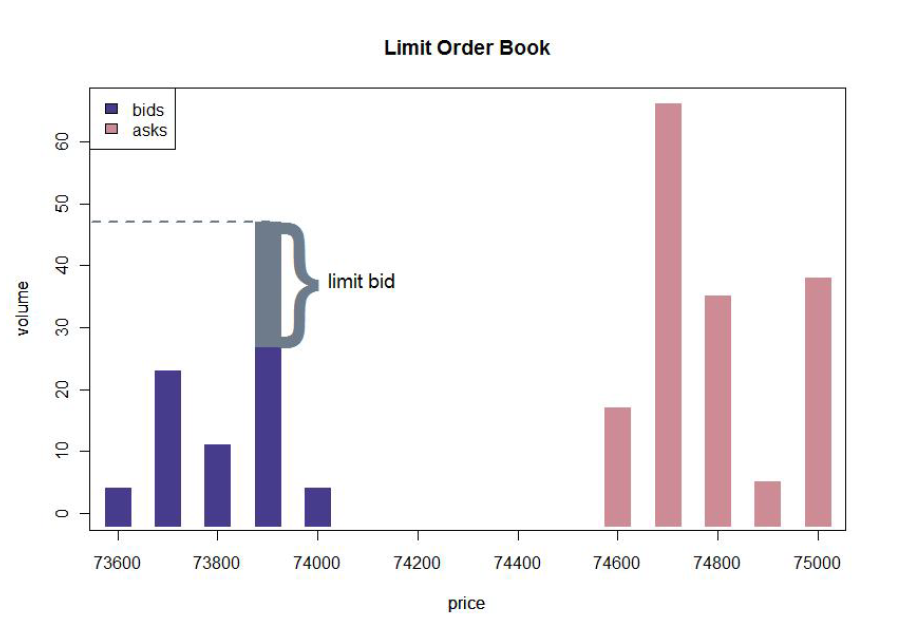
\includegraphics[width=0.9\textwidth]{chapters/chapter_trading_fund/figures/limitbk1.png} 
	   \caption{Limit Order Book---Limit Bid. \label{fig:limbk1}}
	\end{figure}
	
	\begin{figure}[!ht]
	   \centering
	   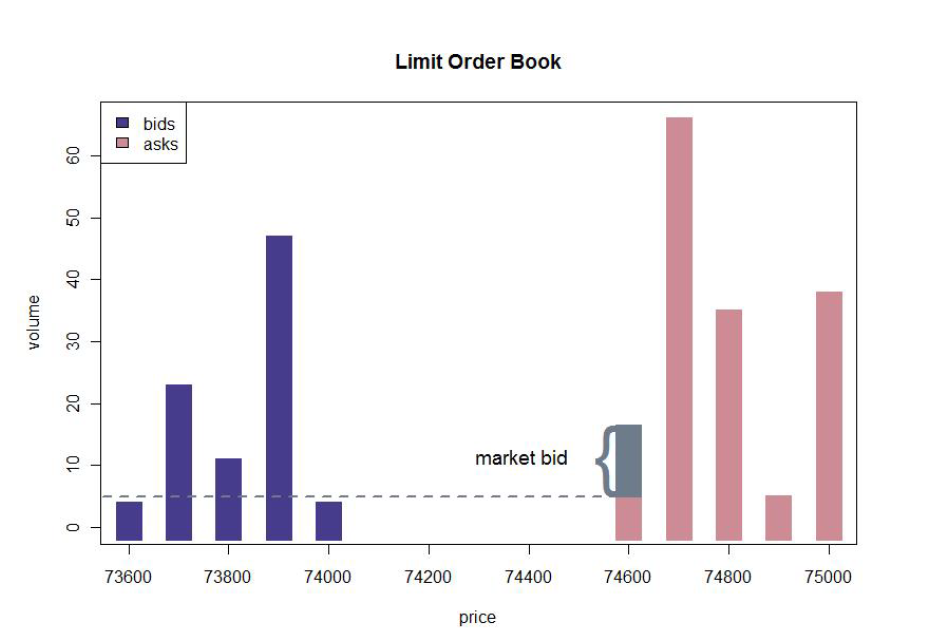
\includegraphics[width=\textwidth]{chapters/chapter_trading_fund/figures/limitbk2.png} 
	   \caption{Limit Order Book---Marketable Bid. \label{fig:limbk2}}
	\end{figure}
	
	\begin{figure}[!ht]
	   \centering
	   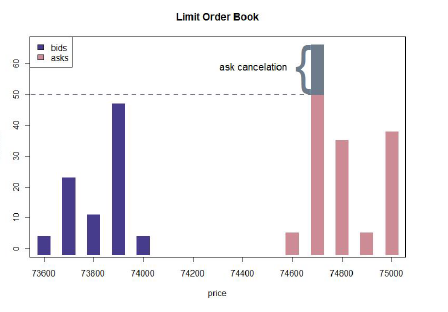
\includegraphics[width=\textwidth]{chapters/chapter_trading_fund/figures/limitbk3.png} 
	   \caption{Limit Order Book---Ask Cancellation. \label{fig:limbk3}}
	\end{figure}


Limit orders make up a significant percentage (70\%) of stock market trading activity. The main advantage of a limit order is that there is no price risk associated to it, that is, when the order is executed the limit price is the maximum (for a buy order) or minimum (for a sell order) price that will be achieved. But if the limit order is not marketable, the execution is not guaranteed and the time to get an order executed depends on various market factors. The trade-off between limit orders and marketable orders depends on the investor's need for immediate liquidity and the fill probability of limit orders. The limit price chosen (how deep in the order book is the order placed) as well as the amount of liquidity ahead of the submitted order (how many shares will need to trade before the order gets executed following, for instance, a price/time priority order matching of the exchange) affect both the order fill probability and its expected time to fill. These two metrics are of particular relevance for execution algorithms and will be studied in more depth later. 


The execution of limit orders does affect how the quotes are posted and are updated. If the size of a market order exceeds the number of shares available at the top of book, it is usually split and is executed at consecutive order book levels until the order is filled. Market orders are usually restricted to be filled within a day and order placed after the markets close might be entered the next day.\footnote{Depending on the Time-in-Force selected} \twomedskip


\noindent\textbf{Order Types:} The diversity of order types is a key component of continuous double auction electronic markets. Order types allow participants to express precisely their intentions with regards to their interaction with the market via the limit order book. Over time, in an effort to cater to sophisticated electronic traders, exchanges around the world have raced to offer ever more complex order types. Here, we will just provide a brief description of some, besides the market and limit orders that were already mentioned:

\begin{itemize}
\item Peg: Specify a price level at which the order should be continuously and automatically repriced. For instance, an order pegged to the bid price will be automatically repriced as a higher price limit order, each time the market bid price ticks up. This order type is particularly used for midpoint executions in non-displayed markets. One would think that pegging order has the additional advantage of improving the queue priority of the order when it is repriced since this process is done directly by the exchange. That turns out not to be true. Managing peg orders is the responsibility of a separate component at the exchange and its interaction speed with the order book is usually slower than that of ultra-low-latency operators.

\item Iceberg: Limit order with a specified display quantity. In order to prevent information leakage to other market participants, a trader desiring to buy or sell a large quantity at a given price might elect to use an iceberg order with a small display size. For instance, for an order to buy 100,000 shares at \$20 with a display size of 2,000 shares. Only 2,000 shares would be displayed in the order book. Once that quantity is executed, the order would automatically reload another 2,000 shares at \$20, and so on, until the full quantity is executed. Note that for iceberg orders, only the visible quantity has time priority and once that quantity has been executed the new tip of the iceberg will be placed at the back of the queue.

\item Hidden: While they are available to trade, these orders are not directly visible to other market participants in the central limit order book. 

\item Stop: These orders are also not visible, but additionally are not immediately entered in the limit order book. They only become active once a certain price (known as the Stop Price) is reached or passed. They then enter the order book as either limit or market order depending on the user setup.

\item Trailing stop: These orders function like stop orders, but the stop price is set dynamic rather than static (for instance: $-3\%$ from previous close).

\item All-or-None: Specifically, request a full execution of the order. If the order is for 1500 shares but only 1000 are being offered, it will not be executed until the full quantity is available.

\item On-Open: Specifically, request an execution at the open price. It can be limit-on-open or market-on-open.

\item On-Close: Specifically, request an execution at the close price. It can be limit-on-close or market-on-close.

\item Imbalance only: Provide liquidity intended to offset on-open/on-close order/imbalances during the opening/closing cross. These generally are limit orders.

\item d-Quote: Special order type on the NYSE mainly used during the close auction period.

\item Funari: Special order type on the Tokyo Stock Exchange which allows limit orders placed in the book during the continuous session to automatically enter the closing auction as market orders. 
\end{itemize}


As described above, there exist a wide variety of orders types offered by different exchanges to facilitate various types of trading activities. Two additional common order types used to automate interactions with the LOB are stop-limit orders and trailing-stop orders. The former is typically used to trade a security at a specified limit price once it is traded through a given stop price. If the stock declines in value and trades below or at the stop price, the order will become a limit order rather than a market order. Trailing-stop orders follow a similar objective but the stop price trails the best bid or ask by a certain percentage. These order types are primarily used by traders as a protection against sudden adverse market moves. \twomedskip


\noindent\textbf{Validity of Instructions:} In addition to conditions on price, it is possible to add conditions on the life duration of the order known as Time-in-Force (TIF). The most common types of TIF instructions include Day orders which are valid for the full duration of the trading session, Extended Day orders allow trading in extended hours, and Good-Till-Cancel (GTC) orders will be placed again on the exchange the next day with similar instructions if they were not completely filled. More sophisticated market participants aiming at achieving greater control over their executions tend to also favor Immediate-or-Cancel (IOC) and Fill-or-Kill (FOK) Time-in-Force instructions. An IOC order will get immediately canceled back to the sender after reaching the matching engine if it does not get an immediate fill, and in case of a partial fill, the unfilled portion will be canceled, thus preventing it from creating a new price level in the order book. In a Fill-or-Kill scenario, the order gets either filled in its entirety or does not get filled at all. This instruction is particularly popular with high frequency market makers and arbitrageurs for which partial fills might result in unwanted legging risk as discussed in Chapter~\ref{ch:stat_ts} on pairs trading.

Finally, it is worth mentioning that some exchanges as well as alternative venues offer the ability of specifying minimum fill sizes. This means that a limit order which might be eligible for a fill due to an incoming order at the same price level, only receives a fill if the incoming order is larger than a pre-specified number of shares or notional value. This type of instruction is used by market participants as a way of minimizing the number of small fills which carry the risk of excessive information dissemination. This happens, in particular, in dark pools, where they can be used to detect the presence of larger limit orders that would be otherwise not visible to market participants.  \label{in:cont_trade2}


% The Closing Auction
\subsection{The Closing Auction} \label{in:close2}

The Closing Auction tends to be the most popular call auction for a variety of reasons. First, it is the last opportunity (unless one engages in the highly risky practice of off-hours trading) for market participants to transact in a relatively liquid environment, before being exposed to the overnight period (when new information accumulates, but trades cannot easily take place). Second, with the increase in passive investment strategies, providing investors with replication of a predetermined benchmark index, the closing auction has become a particularly relevant price setting event. For most passive funds, the net asset value (NAV) is based on close prices of the underlying assets. For those reasons, the closing auction has become extremely important to many investors. From an execution standpoint, it is a major liquidity event that must be handled carefully.


The mechanics of the closing auction are in most part similar to the ones described above for the open auction. The major differences across countries (and sometimes across exchanges within a country) are in the order submission times. Some countries, such as the U.S., have order submissions start and end before the continuous session is over (see Table~\ref{tab:NASDAQclose} and Table~\ref{tab:NYSEclose}), while some other markets have two non-overlapping continuous and close order submission sessions.

	\begin{table}[!ht]
   	\centering
   	\caption{Nasdaq Closing Cross\label{tab:NASDAQclose}}
   	\begin{tabular}{ll} 
	3:55 p.m. EST & Dissemination of imbalance information begins  \\ \hline
	3:55 p.m. EST & Cutoff for entry/amend/cancel of MOC orders\\ \hline
	3:58 p.m. EST & Freeze period - LOC orders cannot be added/canceled  \\ 
	 & OI orders offsetting the imbalance are still accepted   \\ \hline	
	4:00 p.m. EST & The Closing Cross occurs		
  	 \end{tabular}
	\end{table}	


	\begin{table}[!ht]
   	\centering
   	\caption{NYSE Closing Cross\label{tab:NYSEclose}}
   	\begin{tabular}{ll} 
	3:50 p.m. EST & Cutoff for MOC/LOC order entry and modifications  \\ 
     	& Dissemination of imbalance information begins \\
	& Closing Offset orders can be entered until 4:00 p.m.  \\ \hline	 
	3:55 p.m. EST &  Dissemination of d-quote imbalance information\\ \hline
	3:58 p.m. EST & Cutoff for MOC/LOC cancellation for legitimate error \\ \hline
	3:59:50 p.m. EST & Cutoff for d-Quote order entry and modification \\ \hline
	4:00 p.m. EST & The Closing Auction starts \\ \hline
	4:02 p.m. EST & DMM can automatically process auctions not yet complete
   	\end{tabular}
	\end{table}	


	\begin{table}[!ht]
  	\centering
   	\caption{London Stock Exchange Sessions Times\label{tab:LSEclose}}
   	\begin{tabular}{ll} 
	7:00-7:50 a.m. GMT & Pre-Trading  \\ \hline
	7:50-8:00* a.m. GMT & Opening Auction Call\\ \hline
	*8:00-12:00 p.m. GMT & Regular Trading \\ \hline
	12:00-12:02* p.m. GMT & Periodic Call Auction \\ \hline
	*12:02-4:30 p.m. GMT & Regular Trading \\ \hline
	4:30-4:35* p.m. GMT & Closing Auction Call \\ \hline
	*4:35-4:40 p.m. GMT & Closing Price Crossing \\ \hline	
	4:40-5:15 p.m. GMT & Post-Close Trading
   	\end{tabular}
	\begin{minipage}[t]{1\textwidth}
	\small{*Each auction end time is subject to a random 30 second uncross period.\\}
	\small{An additional intraday auction call takes place every 3rd Friday of each month for stocks underlying FTSE 100 index options, and the 3rd Friday of every quarter for stocks underlying FTSE 100/250 Index Futures to determine the EDSP (Exchange Delivery Settlement Price). The settlement price is determined as the index value derived from the individual constituents intraday auction taking place between 10 a.m. and 10:15 a.m. and during which the electronic continuous trading is suspended. Using a call auction ensures the settlement price for these contracts is more representative of a fair market price.}
	\end{minipage}   
	\end{table}	

An aspect of the NYSE is the presence of floor brokers operating in an agency capacity for their customers. They play a particular role during the close auction thanks to their ability to handle discretionary electronic quote orders (known as ``d-Quote'' orders) that offer more flexibility than traditional market-on-close (MOC) and limit-on-close (LOC) orders. The main advantage of d-Quote orders is their ability to bypass the 3:45 pm cutoff and be submitted or canceled until 3:59:50 pm. This allows large institutional investors to remain in control of their orders almost until the end of the continuous session, by delaying the decision of how much to allocate to the auction. They can therefore react to larger volume opportunities based on the published imbalance. They can also minimize the information leakage by not being part of the early published imbalance while there is still significant time in the continuous session for other participants to drive the price away.  Since there is no restriction on the side of d-Quote orders submission, it is possible to see the total imbalance sign flip once the d-Quotes are added to the publication at 3:55 pm, creating opportunities for other market participants to adjust their own close trading via d-Quotes or change their positioning in the continuous session. \label{in:fund_trade2} \label{in:close3}



% Taxonomy of Data for Algorithmic Trading Research
\section{Taxonomy of Data used in Algorithmic Trading }

Running a successful trading operation requires availability of different data sets. Data availability, storage, management, cleaning are some of the most important aspects of a functioning trading business and the core of any research environment. The amount of data and the complexity of maintaining such a ``Data Lake'' can be daunting and very few  excel at this aspect. In this section, we will review the most important data sets and their role in algorithmic trading research. \label{in:data_related1} \label{in:taxonomy}


%%%%%%%%%%%%%%%%%%%%%%%%%
%%%%%%%%%%%%%%%%%%%%%%%%%
\begin{comment}
Historical market data available to researchers and practitioners alike but varied in degrees of granularity over time. From daily trade data (closing price and volume), to tick-by-tick trade and quote data (also known as TAQ data), to full message data, the progression in granularity not only reflects the focus in intraday trading complexity but also opens up the way for more advanced strategies. 

Initially researchers studying the dynamic of LOB had to be content with Trades and Quotes (TAQ) data which provide a time-stamped sequence of trades (Market Orders) and updates in the price and depth of bid and ask quotes. No other information beyond the best bid and the best offer was made available. Also, the updates contained changes at the two best quotes and were aggregated. The aggregation was clearly a limiting factor as one could not discern the kind of events that led to the changing status of the book. The level II data that became available is a time-stamped sequence of trades and quotes for the top 5-levels of the LOB. This data is little deeper than TAQ data, but was still in aggregated form. But recently made available level III data contains time-stamped sequence of all (except for the submission of hidden orders) events that occur in the LOB. Every order is identified by a unique order-id and thus it can be tracked through its lifetime.\footnote{Level III data has been available for years to firm subscribing and storing the raw binary exchange format (pcap) and the re-building the orderbook sequentially from there for their research. It is still the main method used for HFT research. One recently this data became available historically to a broader subset of users and researchers} \twomedskip

\end{comment}
%%%%%%%%%%%%%%%%%%%%%%%%%
%%%%%%%%%%%%%%%%%%%%%%%%%


% Reference Data
\subsection{Reference Data} 

While often overlooked, or merely considered as an afterthought in the development of a research platform,\footnote{More details are presented in a further chapter on research environment} reliable reference data is the key foundation of a robust quantitative strategy development. The experienced practitioner may want to skip this section, however we encourage the neophyte to read through the tedious details to get a better grasp of the complexity at hand.


\begin{itemize}
\item \textbf{Trading Universe:} The first problem for the functioning of a trading operation is knowing what instruments will be required to trade on a particular day. The trading universe is an evolving entity that changes daily to incorporate new listings (IPOs), de-listings, etc. To be able to just trade new instruments, there are several pieces of information that are required to have in multiple systems. Market Data must be made available, and some static data needs to be set or guessed to work with existing controls, parameters for the various analytics need to be made available or sensibly defaulted. For research, in particular quantitative strategies, knowing when a particular stock no longer trades is important to avoid issues like survivor bias.
 
 
\item \textbf{Symbology Mapping:} ISIN, SEDOL, RIC, Bloomberg Tickers, \dots 
%\par\vspace{\baselineskip}

Quantitative strategies often leverage data from a variety of sources. Different providers key their data with different instrument identifiers depending on asset class or regional conventions, or sometimes use their own proprietary identifiers (e.g. Reuters Identification Code---RIC, Bloomberg Ticker). Therefore, symbology mapping is the first step in any data merging exercise. Such data is not static. One of the symbols can change on a given day and others remain unchanged for some time, complicating historical data merges.


It is important to note that such mapping needs to persist as point-in-time data and allow for historical ``as of date'' usage, requiring the implementation of a bi-temporal data structure. Over the course of time, some instruments undergo ticker changes (for example, from ABC to EDF on a later $T_0$) not necessarily without any particular change on the underlying asset. In such cases, market data recorded day-by-day in a trade database will change from being keyed on ABC to being keyed on EDF after the ticker change date $T_0$. This has implications for practitioners working on datasets to build and backtest quantitative strategies. The symbology mapping should allow for both backward and forward handling of the changes.


For instance, in the simple example mentioned below, in order to efficiently backtest strategies over a period of time spanning $T_0$, a robust mapping is needed, so that it will allow to seamlessly query the data for the underlying asset in a variety of scenarios such as:

\begin{itemize}
\item Signal generation: 30-day backward close time series as of date $T < T_0$: \par
{\ttfamily select close from data where date in [T-30,  T], sym = ABC}

\item Signal generation: 30-day backward close time series as of date $T= T_0+10$: \par
{\ttfamily select close from data where date in [T$_0$ - 20, T$_0$ + 10], sym = EDF}

\item Position holding: 30-day forward close time series as of date $T= T_0-10$: \par
{\ttfamily select close from data where date in [T$_0$ - 10,  T$_0$ + 20], sym = ABC}
\end{itemize}


\item \textbf{Ticker Changes:} For comparable reasons as the ones described above in the Symbology Mapping section, one needs to maintain a historical table of ticker changes allowing to seamlessly go up and down time series data. 


\item \textbf{Corporate Actions Calendars:} This category contains stock and cash dividends (both announcement date and execution date), stock splits, reverse splits, rights offer, mergers and acquisitions, spin off, free float or shares outstanding adjustments, quotation suspension, etc.


Corporate actions impact the continuity of price and volume time series and, as such, must be recorded in order to produce adjusted time series. The most common events are dividend distributions. On the day the dividend is paid, the corresponding amount is removed from the stock price, creating a jump in the price time series. The announcement date might also coincide with the stock experiencing more volatility as investors react to the news. Consequently, recording these events proves to be valuable in the design of quantitative strategies as one can assess the effect of dividends announcement or payment on performance, and decide to either not hold a security that has an upcoming dividend announcement or, conversely, to build strategies that look to benefit from the added volatility. 


Another type of corporate events generating discontinuity in historical time series are stock splits or reverse splits and right offers. When the price of a stock becomes too low or too high, a company may seek to split it to bring the price back to a level that is more conducive to liquid trading on exchanges.\footnote{A very low price creates trading frictions as the minimum price increment might represent a large cost relative to the stock price. A very high price might also deter retail investors from investing into a security as it requires them to deploy too much capital per unit.} When a stock experiences a 2:1 split, everything else being equal, its price will be halved and hence, its volume will double. In order to prevent the time series to show discontinuity, all historical data will then need to be adjusted backward to reflect the split.


Mergers \& Acquisitions and Spin-offs are also regular events in the lifecycle of corporations. Their history needs to be recorded in order to account for the resulting changes in valuation that might affect a given ticker(s). These situations can also be exploited by trading strategies known as Merger Arbitrage.


Stock quotations can be suspended as a cooling mechanism (often at the request of the underlying company) to prevent excess price volatility when significant information is about to be released to the market. Depending on the circumstance, the suspension can be temporary and intraday, or can last for extended periods of time if the market place allows it.\footnote{For instance, it was the case for a large number of companies in China in 2016.} Suspensions result in gaps in data and are worth keeping track of, as they can impact strategies in backtesting (inability to enter or exit a position, uncertainty in the pricing of composite assets if a given stock has a significant weight in ETFs or Indexes, etc.). Some markets will also suspend trading if the price swings more than a predefined amount (limit up / limit down situations), either for a period of time or for the remainder of the trading session.


\item \textbf{Static Data:} Country, sector, primary exchange, currency and quote factor. %\par\vspace{\baselineskip}


Static data is also relevant for the development of quantitative trading strategies. In particular, country, currency and sector are useful to group instruments based on their fundamental similarities. A well known example is the usage of sectors to group stocks in order to create pairs trading strategies. It is worth noting that there exist different types of sector classifications (e.g. GICS\textsuperscript\textregistered from S\&P, ICB\textsuperscript\textregistered from FTSE) offering several levels of granularity,\footnote{The Global Industry Classification Standard (GICS\textsuperscript\textregistered) structure consists of 11 sectors, 24 industry groups, 68 industries and 157 sub-industries. An example of this hierarchical structure would be: Industrials / Capital Goods / Machinery / Agricultural \& Farm Machinery.} and that different classifications might be better suited to different asset classes or countries. The constituents of the Japanese index TOPIX, for instance, are classified into 33 sectors that are thought to better reflect the fundamental structure of the Japanese economy and the existence of large diversified conglomerates. 


Maintaining a table of the quotation currency per instrument is also necessary in order to aggregate positions at a portfolio level. Some exchanges allow the quotation of prices in currencies different from the one of the country in which the exchange is located.\footnote{For example, Jardine Matheson Holdings quotes in USD on the Singapore exchange while most of the other securities quote in Singapore Dollars.} Additionally, thus, the Quote Factor associated with the quotation currency data needs to be stored. To account for the wide range of currency values and preserve pricing precision, market data providers may publish FX rates with a factor of 100 or 1000. Hence, to convert prices to USD one needs to multiply by the quote factor: usd price $=$ local price $\cdot$ fx $\cdot$ quote factor. Similarly, some exchanges quote prices in cents, and the associated quotation currency is reflected with a small cap letter: GBP/GBp, ZAR/ZAr, ILS/ILs, etc.


\item \textbf{Exchange Specific Data:}  Despite the electronification of markets, individual exchanges present a variety of differences that need to be accounted for when designing trading strategies. The first group of information concerns the hours and dates of operation:

\begin{itemize}
\item Holiday calendar: As not all exchanges are closed on the same day, and trading days they are off do not always fully follow the country's public holidays, it is valuable to record them, in particular in the international context. Strategies trading simultaneously in several markets and leveraging their correlation, may not perform as expected if one of the markets is closed while others are open. Similarly, execution strategies in one market might be impacted by the absence of trading in another market (for instance, European equity markets volume tends to be 30\% to 40\% lower during U.S. market holidays).

\item Exchange sessions hours: These seemingly trivial data points can get quite complex on a global scale. What are the different available sessions (Pre-Market session, Continuous core session, After-Hour session, etc.)? What are the auction times as well as their respective cutoff times for order submission? Is there a lunch break restricting intraday trading? And if so, are there auctions before and after the lunch break?  The trading sessions in the futures markets sessions can also be quite complex with multiple phases, breaks, as well as official settlement times that may differ from the closing time and have an effect on liquidity.

In Indonesia, for instance, markets have different trading hours on Fridays. Monday through Thursday the Indonesia Stock Exchange (IDX) is open from 9:00~a.m. to 12:00~p.m., and then, from 1:30~p.m. to 4:00~p.m.. On Fridays, however, the lunch break is one hour longer and stretches from 11:30~a.m. to 2:00~p.m.. This weekday effect is particularly important to consider when building volume profiles as discussed in Chapter~\ref{ch:stat_ts}.

Along with local times of operation, it is necessary to consider eventual Daylight Saving Time (DST) adjustments that might affect the relative trading hours of different markets (some countries do not have DST adjustment at all, while for countries that do have one, the dates at which it applies are not always coordinated). Usually, DST starts about two weeks prior to its start in Europe, bringing the time difference between New York and London to four hours instead of five hours. This results in the volume spike in European equities associated to the U.S. market open being one hour earlier, requiring adjustment of volume profiles used for trading executions.

Some exchanges may also adjust the length of trading hours during the course of the year. In Brazil for instance, the Bovespa trading hours are 10:00~a.m. to 6:00~pm. from October to March, but an hour shorter (10:00~a.m. to 5:00~p.m.) from April to September to be more consistent with U.S. market hours. Finally, within one country there might also exist different trading hours by venues as it is the case in Japan where the Nagoya Stock Exchange closes 30~minutes after the major Tokyo Stock Exchange.

\item Disrupted days: Exchange outages or trading disruptions, as well as market data issues, need to be recorded so they can be filtered out when building or testing strategies as the difference in liquidity patterns or the lack of data quality may likely impact the overall outcome.
\end{itemize}


Additionally, exchanges also have specific rules governing the mechanics of trading, such as:
        \begin{itemize}
        \item Tick Size: The minimum eligible price increment. This can vary by instrument, but also change dynamically as a function of the price of the instrument (e.g. stocks under \$1 can quote in increments of \$0.0001, while above that price the minimum quote increment is \$0.01).
        \item Trade and Quote lots: Similar to tick sizes, certain exchanges restrict the minimum size increment for quotes or trades.
        \item Limit-up and Limit-down constraints: A number of exchanges restrict the maximum daily fluctuations of securities. Usually, when securities reach these thresholds, they either pause trading or can only be traded at a better price than the limit-up limit-down threshold.
        \item Short Sell restrictions: Some markets also impose execution level constraints on short sells (on top of potential locate requirements). For instance, while a long sell order can trade at any price, some exchanges restrict short sells not to trade at a price worse than the last price or not create a new quote that would be lower than the lowest prevailing quote. These considerations are particularly important to keep in mind for researchers developing Long-Short strategies as this impacts the ability to source liquidity.
        \end{itemize}
Because these values and their potential activation threshold can vary over time, one needs to maintain historic values as well, in order to run realistic historical backtests.


\item \textbf{Market Data Condition Codes:} With ever-growing complexity in market microstructure, the dissemination of market data has grown complex as well. While it is possible to store daily data as a single entry per day and per instrument, investors building intraday strategies likely need tick by tick data of all the events occurring in the market place. To help classify these events, exchanges and market data providers attribute so-called condition codes to the trades and quotes they publish. These condition codes vary per exchange and per asset class, and each market event can be attributed to several codes at once. So, to aggregate intraday market data properly and efficiently, and decide which events to keep and which ones to exclude, it is necessary to build a mapping table of these condition codes and what they mean: auction trade, lit or dark trade, canceled or corrected trade, regular trade, off-exchange trade reporting, block-size trade, trade originating from a multi-leg order such as an option spread trade, etc.


For instance, in order to assess accessible liquidity for a trading algorithm, trades that are published for reporting purposes (e.g. negotiated transactions that happened off-exchange) must be excluded. These trades should also not been used to update some of the aggregated daily data used in the construction of trading strategies (daily volume, high, low, \dots). Execution algorithms also extensively leverage the distribution of intraday liquidity metrics to gauge their own participation in auctions and continuous sessions, or in lit versus dark venues, therefore requiring a precise classification of intraday market data. 


\item \textbf{Special Day Calendars:} Over the course of a year, some days present certain distinct liquidity characteristics that need to be accounted for in both execution strategies and in the alpha generation process. The diversity of events across markets and asset classes can be quite challenging to handle. Among the irregular events that affect liquidity in equity markets that need to be accounted for, we can mention the following non-exhaustive list for illustration purposes only: half trading days preceding Christmas and following Thanksgiving in the U.S. or on the Ramadan eve in Turkey, Taiwanese market opening on the weekend to make up for lost trading days during holiday periods, Korean market changing its trading hours on the day of the nationwide university entrance exam, Brazilian market opening late on the day following the Carnival, etc.


There are also special days that are more regular and easier to handle. The last trading days of the months and quarters, for instance, tend to have additional trading activity as investors rebalance their portfolios. Similarly, options and futures expiry days (quarterly/monthly expiry, `Triple Witching'\footnote{Triple witching days happen four times a year on the third Friday of March, June, September and December. On these days, the contracts for stock index futures, stock index options and stock options expire concurrently.} in the U.S., Special Quotations in Japan, etc.) tend to result in excess trading volume and different intraday patterns resulting from hedging activity and portfolios adjustments. Consequently, they need to be handled separately, in particular, when modeling trading volume. As most execution strategies make use of relatively short interval volume metrics (e.g. 30-day or 60-day ADV), one single data point can impact the overall level inferred. Similarly autoregressive models of low order may underperform both on special days and on the days following them. As a result, modelers often remove special days and model normal days first. Then, special days are modeled separately, either independently or using the normal days as a baseline. 


In order to reflect changes in the market and remain consistent with index inclusion rules, most indices need to undergo regular updates of the constituents and the respective weights. The significant indices do so at regular intervals (annually, semi-annually or quarterly) on a pre-announced date. At the close of business of that day, some stocks might be added to the index while others are removed, or the weight of each stock in the index might be increased or decreased. These events, known as index rebalances, are particularly relevant to passive investors who are tracking the index. In order to minimize the tracking error to the benchmark index, investors need to also adjust their holdings accordingly. Additionally, as most funds are benchmarked at the close price, there is an incentive for fund managers to try to rebalance their holdings at a price as close as possible to the official close price, on the day the index rebalance becomes effective. As a result, on these days, intraday volume distribution is significantly skewed toward the end of day and requires some adjustment in the execution strategies.


It is worth noting that a special day calendar usage needs not be limited to the country where the event occurs. On days when the U.S. Equities market is closed, there is usually also a significant drop in volume traded in European markets, so it is always valuable to investigate the cross market effect of special days.


\item \textbf{Futures-specific Reference Data:} Futures contracts present particular characteristics requiring additional reference data to be collected. One of the core differences of futures contracts compared to regular stocks is the fact that instruments have an expiry date, after which the instrument ceases to exist. For the purpose of backtesting strategies, it is necessary to know which contract was live at any point in time through the use of an expiry calendar, but also which contract was the most liquid, for instance, equity index futures tend to be the most liquid, for the first contract available (also known as front month), while energy futures such as oil tend to be more liquid for the second contract. While this may appear to be trivial, when building a trading strategy and modeling price series, it is particularly important to know which contract carries the most significant price formation characteristics and what is the true liquidity available in order to estimate transaction costs to properly estimate the market impact. 


The task of implementing a futures expiry calendar is further complicated by the fact there is no real standardized frequency that applies across markets. For instance, European equity index futures tend to expire monthly, while U.S. index futures expire quarterly. Some contracts even follow an irregular cycle through the course of the year as it is the case for grain futures (e.g. wheat) that were originally created for hedging purposes and as a result have expiry months that follow the crop cycle.\footnote{U.S. Wheat Futures expire in March, May, July, September and December.}


The fact futures contracts expire on a regular basis has further implications in terms of liquidity. As investors holding these contracts, they want to maintain their exposure for longer than the lifespan of the contract, they need to roll over their positions onto the next contract. There is often a noticeable difference in the liquidity of consecutive contracts. For instance, the front contract of the S\&P500 (e.g. ESH8) trades roughly 1.5~million contracts per day in the weeks preceding expiry while the next month contract (ESM8) only trades about 30,000 contracts per day. However, this liquidity relationship will invert in the few days leading to the expiry of the front contract as most investors roll their positions, and the most liquid contract will become the back month contract (see Figure~\ref{fig:FutRoll}). As a result, when computing rolling-window metrics (such as average daily volume for instance), it is necessary to account for potential roll dates that may have happened during the time span. In the example above, a simple 60-day average daily volume on ESM8 taken in early April 2018 would capture a large number of days with very low volume (January-March) owing to the fact the most liquid contract at the time was the ESH8 contract, and would not accurately represent the volume activity of the S\&P500 futures contract. A more appropriate average volume metric to be used as a forward looking value for execution purposes would blend the volume time series of ESH8 prior to the roll date, and ESM8 after the roll date.\footnote{It is worth noting that different contracts 'roll' at different speeds. While for monthly expiry contracts it is possible to see most of the open interest switch from the front month contract to the back month on the day prior to the expiry. For quarterly contracts it is not uncommon to see the roll happen over the course of a week or more, and the front month liquidity vanish several days ahead of the actual expiry. Careful modeling is recommended on a case by case basis.} Additionally, in order to efficiently merge futures positions with other assets in an investment strategy, reference data relative to the quotation of these contracts, contract size (translation between the quotation points and the actual monetary value), currency, etc. must be stored.

	\begin{figure}[!ht]
	\centering
	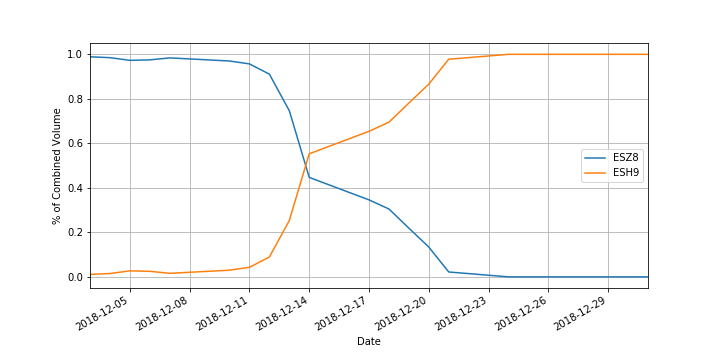
\includegraphics[width=\textwidth]{chapters/chapter_trading_fund/figures/FutRoll.png} 
	\caption{Futures Volume Rolling. \label{fig:FutRoll}}
	\end{figure}

Finally, futures markets are characterized by the existence of different market phases during the day, with significantly different liquidity characteristics. For instance, equity index futures are much more liquid during the hours when the corresponding equities markets are open. However, one can trade during the overnight session if they want to. The overnight session being much less liquid, the expected execution cost tends to be higher, and as such, the various market data metrics (volume profile, average spread, average bid-ask sizes, ...) should be computed separately for each market phase, which requires maintaining a table of the start and end times of each session for each contract. 


\item \textbf{Options-specific Reference Data (Options Chain):} Similar to futures contracts, options contracts present a certain number of specificities for which reference data need to be collected. On top of the similar feature of having a particular expiry date, options contracts are also defined by their strike price. The combination of expiries and strikes is known as the option chain for a given underlier. The ability to map equity tickers to option tickers and their respective strike and expiry dates allow for the design of more complex investment and hedging strategies. For instance, distance to strike, change in open interest of puts and calls, etc. can all be used as signals for the underlying security price. For an interesting article on how deviations in put-call parity contains information about future equity returns, refer to Cremers and Weinbaum (2010)~\cite{weinbaum2010}.


\item \textbf{Market-Moving News Releases:} Macro-economic announcements are known for their ability to move markets substantially. Consequently, it is necessary to maintain a calendar of dates and times of their occurrences in order to assess their impact on strategies and decide how best to react to them. The most common ones are central banks' announcements or meeting minutes, releases about the major economies (FED/FOMC, ECB, BOE, BOJ, SNB), Non-Farm Payrolls, Product and Manufactory Information, Crude Oil Inventories, etc. While these news releases impact the broad market or some sectors, there are also stock specific releases that need to be tracked: earning calendars, specialized sector events such as FDA results for the healthcare and biotech sectors, etc.


\item \textbf{Related tickers:} There is a wide range of tickers that are related to each other, often because they fundamentally represent the same underlying asset. Maintaining a proper reference allows to efficiently exploit opportunities in the market. Some non-exhaustive examples include: primary tickers to composite tickers mapping (for markets with fragmented liquidity), dual listed/fungible securities in US and Canada, American Depository Receipt (ADR) or Global Depository Receipt (GDR), local and foreign boards in Thailand, etc.


\item \textbf{Composite Assets:} Some instruments represent several underlying assets (ETFs, Indexes, Mutual Funds, \dots). Their rise in popularity as investments over time makes them relevant for quantitative strategies. They can be used as efficient vehicles to achieve desired exposures (sector and country ETFs, thematic factor ETFs, \dots), or as cheap hedging instruments, and they can provide arbitrage opportunities when they deviate from their Net Asset Value (NAV). 
In order to be leveraged in quantitative strategies, one needs to maintain a variety of information such as a time series of their constituents and the value of any cash component, the divisor used to translate the NAV into the quoted price, the constituent weights. 


\item \textbf{Latency tables:} This last type of data would only be of interest for developing strategies and for research in the higher frequency trading space. For these, it might be relevant to know the distribution of latency between different data centers as they can be used for more efficient order routing as well as reordering data that may have been recorded in different locations.
\end{itemize}


While the above discussion provides a non-exhaustive list of issues on the reference data available, to build a quantitative research platform, they highlight the challenges that must be taken into account when designing and implementing algorithmic trading strategies. Once in place, a proper set of reference data will allow the quantitative trader to systematically harness the actual content of the types of data (described later) without being caught off-guard by the minutiae of trading.


% Raw Market Data
\subsection{Market Data \label{subsec:marketdata} }

While historically a large swath of modeling for developing strategies was carried out on daily or minute bar datasets, the past fifteen years have seen a significant rise in the usage raw market data in an attempt to extract as much information as possible, and act on it before the opportunity (or market inefficiency) dissipates. Market data, itself, comes in various levels of granularity (and price!) and can be subscribed to either directly from exchanges (known as ``direct feeds'') or from data vendors aggregating and distributing it. The level of detail of the feed subscribed to is generally described as Level~I, Level~II or Level~III market data.\twomedskip


\noindent\textbf{Level I data: Trade and BBO Quotes:} Level I market data is the most basic form of tick-by-tick data. Historically, the level I data feed would only refer to trade information (Price, Size, Time of each trade reported to the tape) but has grown over time into a term generally accepted to mean both trades and top of book quotes. While the trade feed updates with each trade printed on the tape, the quote feed tends to update much more frequently each time liquidity is added to, or removed from the top of book (a rough estimate in liquid markets is the quotes present more updates than the trades by about an order of magnitude). 


In order to build strategies, the timing of each event must be as precise as possible. While the time reported for trade and quotes is the matching engine time at the exchange, most databases also store a reception or record time to reflect the potential latency between the trade event and one being aware that it did happen and be able to start making decision on it. Accounting for this real-world latency is a necessary step for researchers building strategies on raw market data for which opportunities may be very short lived and may be impossible to exploit by participants who are not fast enough.


The Level I data is enough to reconstruct the Best Bid and Offer (BBO) of the market. However, in fragmented markets,\label{in:fragmented} it is also useful to obtain an aggregated consolidated view of all available liquidity at a given price level across all exchanges. Market data aggregator usually provide this functionality for users who do not wish to reconstruct the full order book themselves. 


Finally, it is worth noting that even Level I data contains significant additional information in the form of trade status (cancelled, reported late, etc.) and, trade and quote qualifiers. These qualifiers provide granular details such as whether a trade was an odd lot, a normal trade, an auction trade, an Intermarket Sweep, an average price reporting, in which exchange it took place, etc. These details can be used to better analyze the sequence of events and decide if a given print should be used to update the last price and total volume traded at that point in time or not. For instance, if not processed appropriately, a trade reported to the tape out of sequence could result in a large jump in price because the market may have since moved, and consequently the trade status is an indication that the print should not be utilized as it is.


Capturing raw market data, whether to build a research database or to process it in real-time to make trading decisions, requires significant investments and expert knowledge to handle all the inherent complexity. Hence, one should carefully consider the trade-off between the expected value that can be extracted from the extra granularity, and the additional overhead compared to simpler solutions such as using binned data. \twomedskip


\noindent\textbf{Level II data: Market Depth:}  Level~II market data contains the same information as Level~I, but with the addition of quote depth data. The quote feed displays all lit limit order book updates (price changes, addition or removal of shares quoted) at any level in the book, and for all of the lit venues in fragmented markets. Given the volume of data generated and the decreasing actionable value of quotes updates as their distance to top of book increases, some users limit themselves to the top five or ten levels of the order book  when they collect and/or process the data. \label{in:level2dat1} \twomedskip


\noindent\textbf{Level III data: Full Order View:} Level~III market data---also known as message data---provides the most granular view of the activity in the limit order book. Each order arriving is attributed a unique ID, which allows for its tracking over time, and is precisely known when it is executed, canceled or amended. Similar to Level~II, the dataset contains intraday depth of book activity for all securities in an exchange. Once all messages from different exchanges are consolidated into one single dataset ordered by timestamp, it is possible to build a full (with national depth) book at any moment intraday. For illustration purposes, we take the example of U.S. Level III data and provide a short description below in Table~\ref{tab:level3data}. \label{in:level3dat1}
	\begin{table}[!ht]
	\centering
	\caption{Level III data \label{tab:level3data}}
	\begin{tabular}{lp{0.8\textwidth}} \hline
	Variable & Description \\
	& \\
	Timestamp: & Number of milliseconds after the midnight. \\
	& \\
	Ticker: & Equity symbol (up to 8 characters) \\
	& \\
	Order: & Unique order ID. \\
	& \\
	T & Message type. Allowed values: \newline \begin{minipage}[t]{0.6\textwidth} \begin{itemize} \item ``B''---Add buy order \item ``S''---Add sell order \item ``E''---Execute outstanding order in part \item ``C''---Cancel outstanding order in part \item ``F''---Execute outstanding order in full \item ``D''---Delete outstanding order in full \item ``X''---Bulk volume for the cross event \item ``T''---Execute non-displayed order \end{itemize} \end{minipage} \\
	& \\
	Shares & Order quantity for the ``B'', ``S'', ``E'', ``X'', ``C'', ``T'' messages. Zero for ``F'' and ``D'' messages. \\
	& \\
	Price & Order price, available for the ``B'', ``S'', ``X'' and ``T'' messages. \newline Zero for cancellations and executions. The last 4 digits are decimal digits. The decimal portion is padded on the right with zeros. The decimal point is implied by position; it does not appear inside the price field. Divide by 10000 to convert into currency value. \\ 
	& \\
	MPID & Market Participant ID associated with the transaction (4 characters) \\
	& \\
	MCID & Market Center Code (originating exchange---1 character) 
	\end{tabular}
	\end{table}
	

While the display and issuance of new ID to the modified order varies from exchange to exchange, a few special types of orders are worth mentioning:
        \begin{enumerate}[1.]
        \item Order subject to price sliding: The execution price could be one cent worse than the display price at NASDAQ; it is ranked at the locking price as a hidden order, and is displayed at the price, one minimum price variation (normally 1 cent) inferior to the locking price. New order ID will be used if the order is replaced as a display order. At other exchanges the old order ID will be used.
        \item Pegged order: Based on NBBO, not routable, new timestamp given upon re-pricing; display rules vary over exchanges.
        \item Mid-point peg order: Non-displayed, can result in half-penny execution.
        \item Reserve order: Displayed size is ranked as a displayed limit order and the reserve size is behind non-displayed orders and pegged orders in priority. The minimum display quantity is 100 and this amount is replenished from the reserve size when it falls below 100 shares. A new timestamp is created and the displayed size will be re-ranked upon replenishment.
        \item Discretionary order: Displayed at one price while passively trading at a more aggressive discretionary price. The order becomes active when shares are available within the discretionary price range. The order is ranked last in priority. The execution price could be worse than the display price.
        \item Intermarket sweep order: Order that can be executed without the need for checking the prevailing NBBO.  
        \end{enumerate}


The richness of the dataset allows sophisticated players, such as market makers, to know not only the depth of book at a given price and the depth profile of the book on both sides, but more importantly the relative position of an order from the top position of the side (buy or sell).Among the most common granular microstructure behaviors studied with Level III data, we can mention:
        \begin{itemize}
        \item The pattern of inter-arrival times of various events.
        \item Arrival and cancellation rates as a function of distance from nearest touch price.
        \item Arrival and cancellation rates as a function of other available information, such as in the queue on either side of the book, order book imbalance, etc.
        \end{itemize}
Once modeled, these behaviors can, in turn, be employed to design more sophisticated strategies by focusing on trading related questions:
        \begin{itemize}
        \item What is the impact of market order on the limit order book?
        \item What are the chances for a limit order to move up the queue from a given entry position?
        \item What is the probability of making the spread?
        \item What is the direction of the price movement in short duration?
        \end{itemize}


As illustrated by the diversity and granularity of information available to traders, markets mechanics have grown ever more complex over time, and a great deal of peculiarities (in particular at the reference data level) need to be accounted for in order to design robust and well performing strategies. The proverbial devil is always in the details when it comes to quantitative trading but while it might be tempting to go straight to the most granular source of data, in practice---with the exception of truly high frequency strategies---most practitioners build their algorithmic trading strategies relying essentially on binned data. This simplifies the data collection and handling processes and also greatly reduces the dimension of the datasets so one can focus more on modeling rather than data wrangling. Most of the time series models and techniques described in subsequent chapters are suited to daily or binned data.



% Market Data Derived Statistics
\subsection{Market Data Derived Statistics}

Most quantitative strategies even the higher frequency strategies that leverage more and more granular data also leverage derived statistics from the binned data, such as daily data. Here we give a list of the most common ones used by practitioners and researchers alike. \twomedskip


\noindent\textbf{Daily Statistics} \twomedskip

The first group represents the overall trading activity in the instrument: 

\begin{itemize}
\item \emph{Open, High, Low, Close (OHLC) and Previous Close Price:} The OHLC provides a good indication of the trading activity as well as the intraday volatility experienced by the instrument. The distance traveled between the lowest and highest point of the day usually gives a better indication of market sentiment than the simple close-to-close return. Keeping the previous close value as part of the same time series is also a good way to improve computation efficiency by not having to make an additional database query to compute intraday return and overnight gap. The previous close needs, however, to be properly adjusted for corporate actions and dividends. 


\item \emph{Last trade before close (Price/Size/Time):} It is useful in determining how much the close price may have jumped in the final moments of trading, and consequently, how stable it is as a reference value for the next day.


\item \emph{Volume:} It is another valuable source of trading activity indicator, in particular when the level jumps from long term average. It is also worth collecting the volume breakdown between lit and dark venues, in particular for execution strategies.


\item \emph{Auctions volume:} Depending on the exchange, there can be multiple auctions in a day (Open, Close, Morning Close and Afternoon Open - for markets with a lunch break -, as well as adhoc liquidity or intraday auctions). Owing to their liquidity aggregation nature, they can be considered as a valuable price discovery event when significant volume prints occur.


\item \emph{VWAP:} Similar to the OHLC, the intraday VWAP price gives a good indication of the trading activity on the day. It is not uncommon to build trading strategies using VWAP time series instead of just close-to-close prices. The main advantage being that VWAP prices represent a value over the course of the day and, as such, for larger orders are easier to achieve through algorithmic execution than a single print.


\item \emph{Short Interest / days-to-cover / utilization:} This dataset is a good proxy for investors positioning. The short pressure might be an indication of upcoming short term moves: a large short interest usually indicates a bearish view from institutional investors. Similarly, the utilization level of available securities to borrow (in order to short) gives an indication of how much room is left for further shorting (when securities become ``Hard to Borrow''), the cost of shorting becomes significantly higher requiring short seller to have strong enough beliefs in the short term price direction. Finally, days-to-cover data is also valuable to assess the magnitude of a potential short squeeze. If short sellers need to unwind their positions, it is useful to know how much volume this represents as a fraction of available daily liquidity. The larger the value, the larger the potential sudden upswing on heavily shorted securities.


\item \emph{Futures data:} Futures markets provide additional insight into the activity of large investors through open interest data, that can be useful to develop alpha strategies. Additionally, financial futures offer arbitrage opportunities if their basis exhibits mispricing compared to one's dividend estimates. As such, recording the basis of futures contracts is worthwhile even for strategies that do not particularly target futures.


\item \emph{Index-level data:} This is also a valuable dataset to collect as a source of relative measures for instrument specific features (Index OHLC, Volatility, \dots). In particular for dispersion strategies, normalized features help identify individual instruments from their benchmarks. 


\item \emph{Options data:} The derivative market is a good source of information about the positioning of traders through open interest and Greeks such as Gamma and Vega. How the broader market is pricing an instrument through implied volatility for instance is of interest.


\item \emph{Asset Class Specific:} There is a wealth of cross-asset information available when building strategies, in particular in Fixed Income, FX, and Credit markets. Among the basic ones, we would note:
        \begin{itemize}
        \item Yield / benchmark rates (repo, 2y, 10y, 30y)
        \item CDS Spreads
        \item US Dollar Index
        \end{itemize}
\end{itemize}


The second group of daily data represents granular intraday microstructure activity and is mostly of interest to intraday or execution trading strategies:
        \begin{itemize}
        \item \emph{Number of trades:} A proxy for the activity level of an instrument, and how continuous it is. Instruments with a low number of trades are harder to execute and can be more volatile. 
        
        \item \emph{Number and frequency of quote updates:} Similar proxy for the activity level.
        
        \item \emph{Top of book size:} A proxy for liquidity of the instrument (larger top of book size make it possible to trade larger order size quasi immediately, if needed).
        
        \item \emph{Depth of book (price and size):} Similar proxy for liquidity.
        
        \item \emph{Spread size (average, median, time weighted average):} This provides a proxy for cost of trading. A parametrized distribution of spread size can be used to identify intraday trading opportunities if they are cheap or expensive.
        
        \item \emph{Trade size (average, median):} Similar to spread size, trade sizes and their distribution are useful to identify intraday liquidity opportunities when examining the volume available in the order book.
        
        \item \emph{Ticking time (average, median):} The ticking time and its distribution is a representation of how often, one should expect changes in the order book first level. This is particularly helpful for execution algorithms for which the frequency of updates (adding/canceling child orders, reevaluating decisions, etc.) should be commensurate with the characteristics of the traded instrument.
        
        These daily level distributions of microstructure variables can be used as start of day estimates in trading algorithms and be updated intraday as additional data flows in through online Bayesian updates.
        \end{itemize}


Finally, the last group of daily data can be derived from the previous two groups through aggregation but is usually stored pre-computed in order to save time during the research phase (e.g. X-day trailing data), or to be used as normalizing values (e.g. size as a percentage of ADV, spread in relation to long-term average, \dots). Some common examples would be:
        \begin{itemize}
        \item $X$-day Average Daily Volume (ADV) / Average auction volume
        \item $X$-day volatility (Close-to-close, Open-to-close, etc.)
        \item Beta with respect to an index or a sector (plain beta, or asymmetric up-days/down-days beta)
        \item Correlation matrix
        \end{itemize}

As a reminder to the reader, aggregated data need to fully support the peculiarities described in the Reference Data section (for instance: the existence of special event days which, if included, can significantly skew intraday distribution of values; mishandling of market asynchronicity resulting in inaccurate computations of key quantities such as beta or correlation, etc.).\twomedskip


\noindent\textbf{Binned Data}\label{in:binned_data}\twomedskip

The first natural extension to daily data sets is a discretization of the day into bins ranging from a few seconds to 30 minutes. The features collected are comparable to the ones relevant for daily datasets (period volume, open, high, low, close, VWAP, spread, etc.), but computed at higher frequency. It is worth mentioning that minute bar data actually underpins the vast majority of microstructure models used in the electronic execution space. Volume and spread profiles, for instance, are rarely built with a granularity finer than one minute to prevent introducing excess noise due to purely market friction. The major advantage of binned-data is that discrete time series methods can be readily used.


These minute bar datasets are also quite popular for the backtesting of low-to-medium frequency trading strategies targeting intraday alpha (short duration market neutral long-short baskets, momentum and mean-reversion strategies, etc.). The main benefit they provide is a significant dimension reduction compared to raw market data (390 rows per stock per day in the U.S. compared to millions for raw data for the liquid stocks), which allows researchers to perform rapid and efficient backtesting as they search for alpha. However, increasing data frequency from daily data to intraday minute bars also present challenges. In particular, relationships that appears to be stable using close-to-close values become much noisier as granularity increases and signals become harder to extract (e.g. drop in correlation between assets, pricing inefficiency moves due to sudden liquidity demand, etc.). Similarly, for less liquid assets with a low trade frequency, there may not be any trading activity for shorter durations, resulting in empty bins.


% Fundamental Data
\subsection{Fundamental Data and other Datasets}

A very large number of quantitative investment strategies are still based on fundamental data, and consequently countless research papers are available to the interested reader describing examples of their usage. Here we will only describe the main classes of existing fundamental data:


\begin{itemize}
\item \textbf{Key ratios:} EPS (Earnings Per Share), P/E (Price-to-Earning), P/B (Price-to-Book Value), \dots. These metrics represent a normalized view of the financials of companies allowing for easier cross-sectional comparison of stocks and their ranking over time.


\item \textbf{Analyst recommendations:} Research analysts at Sell Side institutions spend a great deal of resources analyzing companies they cover, in order to provide investment recommendations usually in the form of a Buy/Hold/Sell rating accompanied by a price target. While individual recommendations might prove noisy, the aggregate values across a large number of institutions can be interpreted as a consensus valuation of a given stock, and changes in consensus can have a direct impact on price.


\item \textbf{Earnings data:} Similarly research analysts also provide quarterly earning estimates that can be used as an indication of the performance of a stock before the actual value gets published by the company. Here, too, consensus values tend to play a larger role. In particular, when the difference between the forecast consensus and the realized value is large (known as earning surprise), as the stock might then experience outsized returns in the following days. Thus, collecting analysts' forecasts as well as realized values can be a valuable source of information in the design of trading strategies.


\item \textbf{Holders:} In some markets, large institutional investors are required to disclose their holdings on a regular basis. For instance, in the U.S., institutional investment managers with over \$100 million in assets must report quarterly, their holdings, to the SEC using Form 13F. The forms are then publicly available via the SEC's EDGAR database. Additionally, shareholders might be required to disclose their holdings once they pass certain ownership thresholds.\footnote{In the U.S., Form 13D must be filed with the SEC within 10 days by anyone who acquires beneficial ownership of more than 5\% of any class of publicly traded securities in a public company.} Sudden changes in such ownership might indicate changes in sentiment by sophisticated investor and can have a significant impact on stock performance.


\item \textbf{Insiders Purchase/Sale:} In some markets, company directors are required by law to disclose their holdings of the company stock as well as any increase or decrease of such holdings.\footnote{In the U.S., officers and directors of publicly traded companies are required to disclose their initial holdings in the company by filing Form 3 with the SEC, as well as Form 4 within 2 days of any subsequent changes. The forms are then publicly available via the SEC's EDGAR database.} This is thought to be an indicator of future stock price moves from the group of people who have access to the best possible information about the company.


\item \textbf{Credit Ratings:} Most companies issue both stocks and bonds to finance their operations. The credit ratings of bonds and the changes over time provide additional insight into the health of a company and are worth leveraging. In particular, credit downgrades resulting in higher funding costs in the future, generally have a negative impact on equity prices.


\item \textbf{And much, much more:} Recent years have seen the emergence of a wide variety of alternative data sets that are available to researchers and practitioners alike.\footnote{For instance, \url{www.orbitalinsight.com} offers daily retail traffic analytics, derived from satellite imagery analysis monitoring over 260,000 parking lots, as well as estimates of oil inventories through satellite monitoring of oil storage facilities.} While it is not possible to make a comprehensive list of all that are available, they can generally be classified based on their characteristics: frequency of publication, structured or unstructured, and velocity of dissemination. The value of such data depends on the objectives and resources of the user (natural language processing or image recognition for unstructured data require significant time and efforts), but also---and maybe more importantly---on the uniqueness of the dataset. As more investors get access to it, the harder it becomes to extract meaningful alpha from it. \label{in:data_related2}
\end{itemize}


% Market Microstructure: Academic Perspective
\section{Market Microstructure: Economic Fundamentals of Trading}\label{in:fund_trade3}\label{in:bidask1}\label{in:micro1}

We provide a brief review of market microstructure, an aptly termed phrase about market making and inventory costs,\label{in:tradecost1} first and then delve into some key operational concepts. We draw upon some key review papers by Madhavan (2000)~\cite{madhavan2000}, Biais, Glosten and Spatt (2005)~\cite{bgs05} and O'Hara (2015)~\cite{ohara15hfmm}. It is the area of finance that studies how the supply and demand of liquidity results in actual transactions and modifies the subsequent state of the market. The core idea is that the efficient market hypothesis,\label{in:efficient} which postulates that the equity price impounds all the information about the equity, may not hold due to market frictions. Algorithmic trading essentially exploits the speed with which investors acquire the information and how they use it along with the market frictions that arise mainly due to demand-supply imbalances. Madhavan (2000)~\cite{madhavan2000} provides a microstructure analysis framework from an informational economics viewpoint. 


\begin{enumerate}[--]
\item Price formation and price discovery: How do prices impound information over time and how do the determinants of trading costs vary?

\item Market Design: How can trading rules affect price formation? 

\begin{comment}
The early focus was on the role of so-called market makers who are professional traders willing to buy or sell equities on demand. Thus, they provide liquidity and facilitate the trading to be done uninterrupted although the demand and supply can arise at irregular intervals. They are active on both sides of the market with bid-ask spread as the return for their role. The spread may be adjusted in response to changes in their inventories. Market makers play an active role in price setting; their primary goal is to maximize the inventory turnover, if they are heavily invested in one side of the market. Thus their deals may at times depart from rational theories. Models developed to study their behavior use stochastic dynamic programming assuming that each deal is based on an auction and with a large number of sequential trading deals, the trading becomes a continuous double-auction process. The prices on both sides of the market are set to optimize the net revenue adjusted for idle inventory costs. The studies on the variability of the bid-ask spread indicate that the volume of trading, riskiness of the asset, price and firm size could be important determinants. Spreads are wider for riskier assets and higher volume stocks generally known to have lower spreads.


The deviation from fundamental values of a stock can arise from asymmetric information or from strategic behaviors of investors and intermediaries. The rules that govern them can influence the frictions and transaction costs arising from the trading process. The revenues of agents supplying liquidity depend on order handling costs, adverse selection costs and inventory costs. 
\end{comment}

Market design generally refers to a set of rules that all players have to follow in the trading process. These include the choice of tick size, circuit breakers\label{in:circ_br} which can halt trading in the event of large price swings, the degree of anonymity and the transparency of the information to market participants, etc. Markets around the world and across asset classes can differ significantly in these types of rules, creating a diverse set of constraints and opportunity for algorithmic traders. Some early research on effects the market design lead to following broad conclusions.

\begin{enumerate}[--]
\item Centralized trading via one single market tends to result in more efficient price discovery with smaller bid-ask spreads. In the presence of multiple markets, the primary markets (such as NYSE, NASDAQ) remain the main sources of price discovery.

\item Despite market participants preference for continuous, automated limit order book markets, theoretical models suggest that multilateral trading approaches such as single-price call auctions are the most efficient in processing diverse information.  

\item Transparency which is broadly classified into pre-trade (lit order book) and post-trade (trade reporting to the public, though at different time lags) is often a trade off. While in theory more transparency should lead to better price discovery, the wide disclosure of order book depth information can lead to thinner posted sizes and wider bid-ask spreads if participants fear revealing their intent and possibly their inventory levels, leading them to favor more off-exchange activity.  
\end{enumerate}
\end{enumerate}

All the above points can be analyzed in light of the rapid growth of high frequency trading (HFT) described earlier in this chapter. O'Hara (2015)~\cite{ohara15hfmm} presents issues related to microstructure in the context of HFT. While the basic tenet that traders may use private information or learn from market data such as orders, trade size, volume, duration between successive trades, etc., has remained the same, the trading is now mostly automated to follow some rules. These rules are based on partly prior information and partly on changing market conditions, monitored through order flows. With the high speed, adverse selection has taken a different role. Some traders may have access to market data milliseconds before others have it and this may allow them to make short term price movements. This would expand the pool of informed traders. Here are some topics for research in microstructure:


\begin{enumerate}[--]
\item With a parent order sliced into several child orders that are sent to market for execution during the course of trading, it is difficult to discern who is the informed trader. Informed traders use sophisticated dynamic algorithms to interact with the market. Retail (uninformed) trades usually cross the spread.

\item More work needs to be done to understand trading intensity in short intervals. Order imbalance is empirically shown to be not related to price levels. 

\item Informed traders may increasingly make use of hidden orders. How these orders enter and exit the markets require further studies. 

\item Traders respond to changing market conditions via revising their quoted prices. The quote volatility can provide a valuable information about the perceived uncertainty in the market.
\end{enumerate}


Although HFT has resulted in more efficient markets, with lower bid-ask spreads, the data related to trade sequences, patterns of cancellations across the fragmented markets require new tools for analysis and for making actionable inference. In this review, we do not present any models explicitly and these will be covered throughout this book. Now keeping in line with the practical perspectives of this book, we highlight some key concepts.


% Liquidity and Market Making
\subsection{Liquidity and Market Making\label{sec:liq_market_making}}

\begin{enumerate}
\item[\textbf{a)}] \textbf{A definition of liquidity:} Financial markets are commonly described as carrying the function of efficiently directing the flow of savings and investments to the real economy to allow the production of goods and services. An important factor contributing to well-developed financial markets is in facilitating liquidity which enables investors to diversify their asset allocation and the transfers of securities at a reasonable transaction cost. 

Properly describing ``liquidity'' often proves to be elusive as there is no commonly agreed upon definition. Black (1971)~\cite{black71} proposes a relatively intuitive description of a liquid market:
\emph{``The market for a stock is liquid if the following conditions hold}:
	\begin{itemize}
	\item \emph{There are always bid and ask prices for the investor who wants to buy or sell small amounts of stock immediately.}
	\item \emph{The difference between the bid and ask prices (the spread) is always small.}
	\item \emph{An investor who is buying or selling a large amount of stock, in the absence of special information, can expect to do so over a long period of time at a price not very different, on average, from the current market price.}
	\item \emph{An investor can buy or sell a large block of stock immediately, but at a premium or discount that depends on the size of the block. The larger the block, the larger the premium or discount.''}
	\end{itemize}
In other words, Black defines a liquid market as a continuous market having the characteristics of relatively tight spread, with enough depth on each side of the limit order book to accommodate instantaneous trading of small orders, and is resilient enough to allow large orders to be traded slowly without significant impact on the price of the asset. This general definition remains particularly well suited to today's modern electronic markets and can be used by practitioners to assess the difference in liquidity between various markets when choosing where to deploy a strategy. \twomedskip

\item[\textbf{b)}] \textbf{Model for Market Friction:} We begin with a model to accommodate the friction in stock price ($P_t$). If $p_t^*$ is the (log) true value of the asset which can vary over time due to expected cash flows or due to variation in the discount rate. Given the publicly available information and the assumption of market efficiency, we have: $p_t= p_t^* + a_t$ and $p_t^*= p_{t-1}^* + \epsilon_t$. Therefore the observed return, $r_t= p_t - p_{t-1}= \epsilon_t + (a_t - a_{t-1})$ can exhibit some (negative) serial correlation, mainly a result of friction. The friction, `$a_t$' can be a function of number of factors such as inventory costs, risk aversion, bid-ask spread, etc. When $a_t= c s_t$, where $s_t$ is the direction of the trade and `$c$' is the half-spread, the model is called Roll model. This can explain the stickiness in returns in some cases.  

\item[\textbf{c)}] \textbf{Different styles of market participants: liquidity takers and liquidity providers:} Liquid financial markets carry their primary economic function by facilitating savings and investment flows as well as allowing investors to exchange securities in the secondary markets. Economic models of financial markets attempt to classify market participants into different categories. These can be broadly delineated as: \twomedskip

\textbf{Informed Traders,} making trading decisions based on superior information that is not yet fully reflected in the asset price. That knowledge can be derived from either fundamental analysis or information not directly available nor known to other market participants. \twomedskip

\textbf{News Traders,} making trading decisions based on market news or announcements and are trying to make profits by anticipating the market's response to a particular catalyst. The electronification of news dissemination offers new opportunities for developing quantitative trading strategies by leveraging text-mining tools such as natural language processing to interpret, and trade on, machine readable news before it is fully reflected in the market prices. %Chapter~\ref{chap:ch_news_an} will detail some of the advances in the field.
 \twomedskip

\textbf{Noise Traders} (as introduced by Kyle (1985)~\cite{kyle1985}), making trading decisions without particular information and at random times mainly for liquidity reasons. They can be seen as adding liquidity to the market through additional volume transacted, but only have a temporary effect on price formation. Their presence in the market allows informed traders not to be immediately detected when they start transacting, as market makers cannot normally distinguish the origin of the order flow between these two types of participants. In a market without noise traders, being fully efficient, at equilibrium each trade would be revealing information that would instantly be incorporated in prices, hereby removing any profit opportunities. \twomedskip

\textbf{Market Makers,} providing liquidity to the market with the intent of collecting profits originating from trading frictions in the market place (bid-ask spread). Risk-neutral market makers are exposed to adverse selection risk arising from the presence of informed traders in the marketplace, and therefore establish their trading decisions mostly based on their current inventory. As such, they are often considered in the literature to drive the determination of efficient prices by acting as the rational intermediaries.  

Generalizing these concepts, market participants and trading strategies can be separated between liquidity providing and liquidity seeking. The former being essentially the domain of market makers whose level of activity, proxied by market depth, is proportional to the amount of noise trading and inversely proportional to the amount of informed trading (Kyle (1985)~\cite{kyle1985}). The latter being the domain of the variety of algorithmic trading users, described before (mutual funds, hedge funds, asset managers, etc.). Given the key role played by market makers in the liquidity of electronic markets, they have been the subject of a large corpus of academic research focusing on their activities. \label{in:bidask2} \twomedskip


\item[\textbf{d)}] \textbf{The objectives of the modern Market Maker:}
In present days, market making can broadly be separated into two main categories based on the trading characteristics. The first one is the provision of large liquidity---known as blocks---to institutional investors, and has traditionally been in the realm of sell-side brokers acting as intermediaries and maintaining significant inventories. Such market makers usually transact through a non-continuous, negotiated, process based on their current inventory, as well as their assessment of the risk involved in liquidation of the position in the future. Larger or more volatile positions generally tend to come at a higher cost, reflecting the increased risk for the intermediary. But they provide the end investor with a certain price and an immediate execution bearing no timing risk that is associated with execution over time. These transactions, because they involve negotiations between two parties, still mostly happen in a manual fashion or over the phone and then get reported to an appropriate exchange for public dissemination.

The second category of market making involves the provision of quasi-continuous, immediately accessible quotes on an electronic venue. With the advent of electronic trading described in the previous section, market makers originally seated on the exchange floors have progressively been replaced by electronic liquidity providers (ELP). The ELPs leverage fast technology to disseminate timely quotes across multiple exchanges and develop automated quantitative strategies to manage their inventory and the associated risk. As such, most ELPs can be classified as high frequency traders. They derive their profits from three main sources: from liquidity rebates on exchanges that offer maker-taker fee structure, from spread earned when successfully buying on the bid and selling on the offer, and from short-term price move favorable to their inventory. 

Hendershott, Brogaard and Riordan (2014)~\cite{hendershott2014} find that HFT activity tends to be concentrated in large liquid stocks and postulate that this can be attributed to a combination of larger profit opportunities emanating from trades happening more often, and from easier risk management due to larger liquidity that allows for easier exit of unfavorable positions at a reasonable cost. \twomedskip


\item[\textbf{e)}] \textbf{Risk management:} In the existing literature on informed trading, it is observed that liquidity supplying risk-neutral market makers are adversely selected by informed traders suddenly moving prices against them. For example, a market maker buy quote tends to be executed when large sellers are pushing the price down, resulting in even lower prices in the near term. This significant potential asymmetry of information at any point in time emphasizes the need for market makers to employ robust risk management techniques, particularly in the domain of inventory risk. For a market maker, risk management is generally accomplished by first adjusting market quotes upward or downward to increase the arrival rate of sellers or buyers and similarly adjusting the inventory in the desired direction. If biasing the quotes does not result in a successful inventory adjustment, the market makers generally employ limit orders to cross the spread.
\end{enumerate}


Ho and Stoll (1981)~\cite{ho1981} introduced a market making model in which the market maker's objective is to maximize profit while minimizing the probability of ruin by determining the optimal bid-ask spread to quote. The inventory held evolves through the arrival of bid and ask orders, where the arrival rate is taken to be a function of bid and ask prices. Their model also incorporates the relevant notion of the size dependence of spread on the market marker's time horizon. The longer the remaining time, the greater potential for adverse move risk for liquidity providers, and vice versa. This is consistent with observed spreads. In most markets, the spread is wider at the beginning of the day, narrowing toward the close. An additional reason annotated for the wider spread right after the beginning of the trading day is due to existence of potentially significant information asymmetry accumulated overnight. As market makers are directly exposed to that information asymmetry, they tend to quote wider spreads while the price discovery process unfolds following the opening of continuous trading, and progressively tighten them as uncertainty about the fair price for the asset dissipates.


Understanding the dynamics of market makers inventory and risk management, and their effect on spreads, has direct implications for the practitioners who intend to deploy algorithmic trading strategies as the spread paid to enter and exit positions is a non-negligible source of cost that can erode the profitability of low alpha quantitative strategies. 


Hendershott and Seasholes (2007)~\cite{hendersea} confirms that market makers' inventories are negatively correlated with previous price changes and positively correlated with subsequent changes. This is consistent with market makers first acting as dampener of buying or selling pressure by bearing the risk of temporarily holding inventory in return for earning the spread and thus potential price appreciation from market reversal. This model easily links liquidity provision and the dynamics of asset prices. 


Finally, it has been observed that there is a positive correlation of market makers inventory with subsequent prices changes, inventories can complement past returns when predicting future returns. Since inventories are not publicly known, market participants use different proxies to infer their values throughout the day. Two commonly used proxies are trade imbalances (the net excess of buy or sell initiated trade volume) and spreads. Trade imbalance aims at signaling trades, either buy initiated or sell initiated, by comparing their price with the prevailing quote. Given market makers try to minimize their directional risk, they can only accommodate a limited amount of non-diversified inventory over a finite period of time. As such, spread sizes, and more particularly their sudden variation, have also been used as proxies for detecting excess inventory from liquidity providers.\label{in:micro2}\label{in:fund_trade4}




%%%%%%%%%%%%%%%%%%%%%%%%%
%%%%%%%%%%%%%%%%%%%%%%%%%
\begin{comment}

In the context of market making, two important price behaviors are relevant to model: momentum and mean-reversion. Both of these price dynamics represent a departure from the pure random walk assumption for asset prices as well as the efficient market hypothesis developed by Eugene Fama that states that asset prices reflect all available information and consequently that past prices cannot predict future performance. Jegadeesh and Titman (1993)~\cite{JeTit1993} identified the potential profitability of momentum in equities documenting the outperformance of strategies that suggest buying stocks that have performed well in the recent past while selling stocks that have performed poorly. CTA funds are among the first to have implemented momentum strategies in a systematic way, in the commodities futures space, both on single and multiple assets (such as baskets of commodities where momentum metrics can be applied either to the single assets or to the relative performance of assets within the basket). 


The most na\"ive momentum strategies rely on simple time series analysis such as price return over a period of time to decide which asset go long (previous positive return) and which asset go short (previous negative return). Other commonly used momentum signals include simple moving averages (MA), moving averages crossovers (of a short-term MA with a longer term MA), exponential weighted moving averages  (EWMA), as well as more sophisticated techniques leveraging machine learning tools. The key characteristic of momentum strategies is their flexibility and relative low complexity. They can be designed at various time intervals (from minutes to months), make use of cross-sectional indicators, be corrected for seasonal effects, and so on. Chapter 2 on Time Series will provide in-depth coverage of techniques that are commonly used by practitioners. In discrete time, the AR(1) process is typically used to model mean-reversion, and it will be described in more details in Chapter 2 as well. 


In continuous time, one well known mean-reverting process is the Ornstein-Uhlenbeck (OU) stochastic process (Uhlenbeck and Ornstein (1930)~\cite{uhlenbeck}). It is described by the following stochastic differential equation:
	\begin{equation} \label{eqn:dxttheta}
	 dX_t = \theta(\mu - X_t)\,dt + \sigma \, dW_t,
	\end{equation}
where $W_t$ is a standard Brownian motion, and $\theta, \sigma$ are positive constants. The value $\mu$ is the long term mean of the process, the coefficient of $dt$ is called the drift, and $\sigma$ is the volatility. One can observe that the drift is negative for $X_t > \mu$ and positive for $X_t < \mu$ , making the process revert towards $\mu$ over time. $\theta$ is commonly known as the rate of mean reversion. While the OU process assumes the volatility $\sigma$ is a constant term, more advanced models with varying volatility allow for behaviors closer to real asset price dynamics. With the increasing availability of ultra-high frequency data, the trading data arrives at a quasi-continuous time scale and the models such OU process have become easily testable.



% RFQ Markets
\subsection{RFQ Markets}

Outside of continuous double auction markets the problem is somewhat simplified and might not require the same layered structured. For instance, RFQ markets can be modeled as single step Markov decision process where one submits a quote (a quantity at a certain price) and receives an execution or not which end the process for this order. The execution policy can then be simply optimized to achieve a desired hit ratio or control inventory risk for instance.


\end{comment}
%%%%%%%%%%%%%%%%%%%%%%%%%
%%%%%%%%%%%%%%%%%%%%%%%%%